\documentclass[12pt, a4paper]{article}

% --- Packages ---
\usepackage[margin=1in]{geometry} % Page margins
\usepackage{amsmath}              % Math formulas
\usepackage{amssymb}              % Math symbols
\usepackage{graphicx}             % Inserting images (SPICE plots, schematics)
\usepackage{booktabs}             % Beautiful tables
\usepackage{caption}              % Caption formatting
\usepackage{float}                % Image placement
\usepackage{hyperref}             % Hyperlinks
\usepackage{fancyhdr}             % Header/Footer
\usepackage{bookmark}             % Bookmarks (fixes rerunfilecheck warning)

% --- Header and Footer ---
\setlength{\headheight}{15pt}
\pagestyle{fancy}
\fancyhf{}
\lhead{Analog IC Design: Assignment-3}
\rhead{Spring 2026, IIIT Hyderabad}
\cfoot{\thepage}

% --- Document Information ---
\title{\textbf{Assignment-3: Noise}\\ \large Analog IC Design (Spring 2026)}
\author{
    \textbf{Chamarthy Madhan Sai Krishna} \\ 
    Roll Number: \texttt{2023102030}
}
\date{Due Date: 10th April 2026}

\begin{document}

\maketitle
\thispagestyle{fancy}

\hrule
\vspace{0.5cm}
\noindent \textbf{Note:} As per the instructions, practice problems from Question 1 are not included in this report.
\vspace{0.5cm}

% ==========================================
% QUESTION 2: RC Circuit
% ==========================================
\section*{2. RC Circuit Noise Analysis}

\subsection*{(a) Derivation of PSD and Output Integrated Noise Power}
The only noise source in this circuit is the thermal noise of the resistor. The input power spectral density (PSD) of the resistor is:
\begin{equation}
    S_{v_{in}}(f) = 4kTR
\end{equation}

The RC low-pass filter has a voltage transfer function $H(s)$:
\begin{equation}
    H(s) = \frac{1}{1 + sRC} \implies |H(j2\pi f)|^2 = \frac{1}{1 + (2\pi fRC)^2}
\end{equation}

The output noise spectral density $S_{v_{out}}(f)$ is the input PSD multiplied by the squared magnitude of the transfer function:
\begin{equation}
    S_{v_{out}}(f) = S_{v_{in}}(f) \times |H(j2\pi f)|^2 = \frac{4kTR}{1 + (2\pi fRC)^2}
\end{equation}

To find the total noise power within a bandwidth from $f_l$ to $f_h$, we integrate the output PSD:
\begin{equation}
    P_{n_{out}} = \int_{f_l}^{f_h} S_{v_{out}}(f) df = \int_{f_l}^{f_h} \frac{4kTR}{1 + (2\pi fRC)^2} df
\end{equation}

Using the standard integral form $\int \frac{1}{1 + (ax)^2} dx = \frac{1}{a} \arctan(ax)$, we get:
\begin{equation}
    P_{n_{out}} = \frac{4kTR}{2\pi RC} \left[ \arctan(2\pi fRC) \right]_{f_l}^{f_h} = \frac{2kT}{\pi C} \left( \arctan(2\pi f_hRC) - \arctan(2\pi f_lRC) \right)
\end{equation}

\vspace{0.5cm}
\textbf{Calculations for $R = 10 \text{ k}\Omega, C = 10 \text{ pF}$:} \\
Assuming room temperature $T = 300 \text{ K}$ and Boltzmann's constant $k \approx 1.38 \times 10^{-23} \text{ J/K}$:
\begin{itemize}
    \item $kT \approx 4.142 \times 10^{-21} \text{ J}$
    \item $RC = (10 \times 10^3) \times (10 \times 10^{-12}) = 10^{-7} \text{ s}$
\end{itemize}

\textbf{Case 1 ($BW = 10 \text{ GHz} - 1 \text{ Hz}$):} \\
Approximating as infinite bandwidth ($f_l \to 0, f_h \to \infty$):
\begin{equation}
    P_{n_{out}} = \frac{2kT}{\pi C} \left( \frac{\pi}{2} - 0 \right) = \frac{kT}{C}
\end{equation}
\begin{equation}
    P_{n_{out}} = \frac{4.142 \times 10^{-21}}{10 \times 10^{-12}} = 4.142 \times 10^{-10} \text{ V}^2 \implies \mathbf{v_{n_{out}} = 20.35 \text{ $\mu$V}}
\end{equation}

\textbf{Case 2 ($BW = 1 \text{ MHz} - 1 \text{ kHz}$):}
\begin{align*}
    2\pi f_hRC &= 2\pi(10^6)(10^{-7}) = 0.2\pi \approx 0.6283 \\
    2\pi f_lRC &= 2\pi(10^3)(10^{-7}) = 0.0002\pi \approx 0.000628
\end{align*}
\begin{equation}
    P_{n_{out}} = \frac{2(4.142 \times 10^{-21})}{\pi(10 \times 10^{-12})} \times \left[ \arctan(0.6283) - \arctan(0.000628) \right]
\end{equation}
\begin{equation}
    P_{n_{out}} = 2.637 \times 10^{-10} \times (0.5610 - 0.0006) = 1.478 \times 10^{-10} \text{ V}^2 \implies \mathbf{v_{n_{out}} = 12.16 \text{ $\mu$V}}
\end{equation}


\subsection*{(b) Noise Simulation Verification}
% Uncomment the lines below and add your screenshot filename
\begin{figure}[H]
    \centering
    
\includegraphics[width=0.8\textwidth]{images/q2_b_1.png} 
    \caption{Noise simulation verifying $v_{n_{out}}$ via LTspice log output.}
\end{figure}

\begin{figure}[H]
    \centering
    
\includegraphics[width=0.8\textwidth]{images/q2_b_2.png} 
    \caption{Noise simulation verifying $v_{n_{out}}$ for the second bandwidth case.}
\end{figure}
\textit{Discussion:} As seen in the attached simulation log, the simulated total RMS noise voltage integrated over the bandwidth closely matches our calculated values ($20.35\text{ }\mu\text{V}$ for Case 1 and $12.16\text{ }\mu\text{V}$ for Case 2), verifying the theoretical derivation up to 2 decimal points.


\subsection*{(c) AC Gain and Noise Spectrum Plots}
\begin{figure}[H]
    \centering
    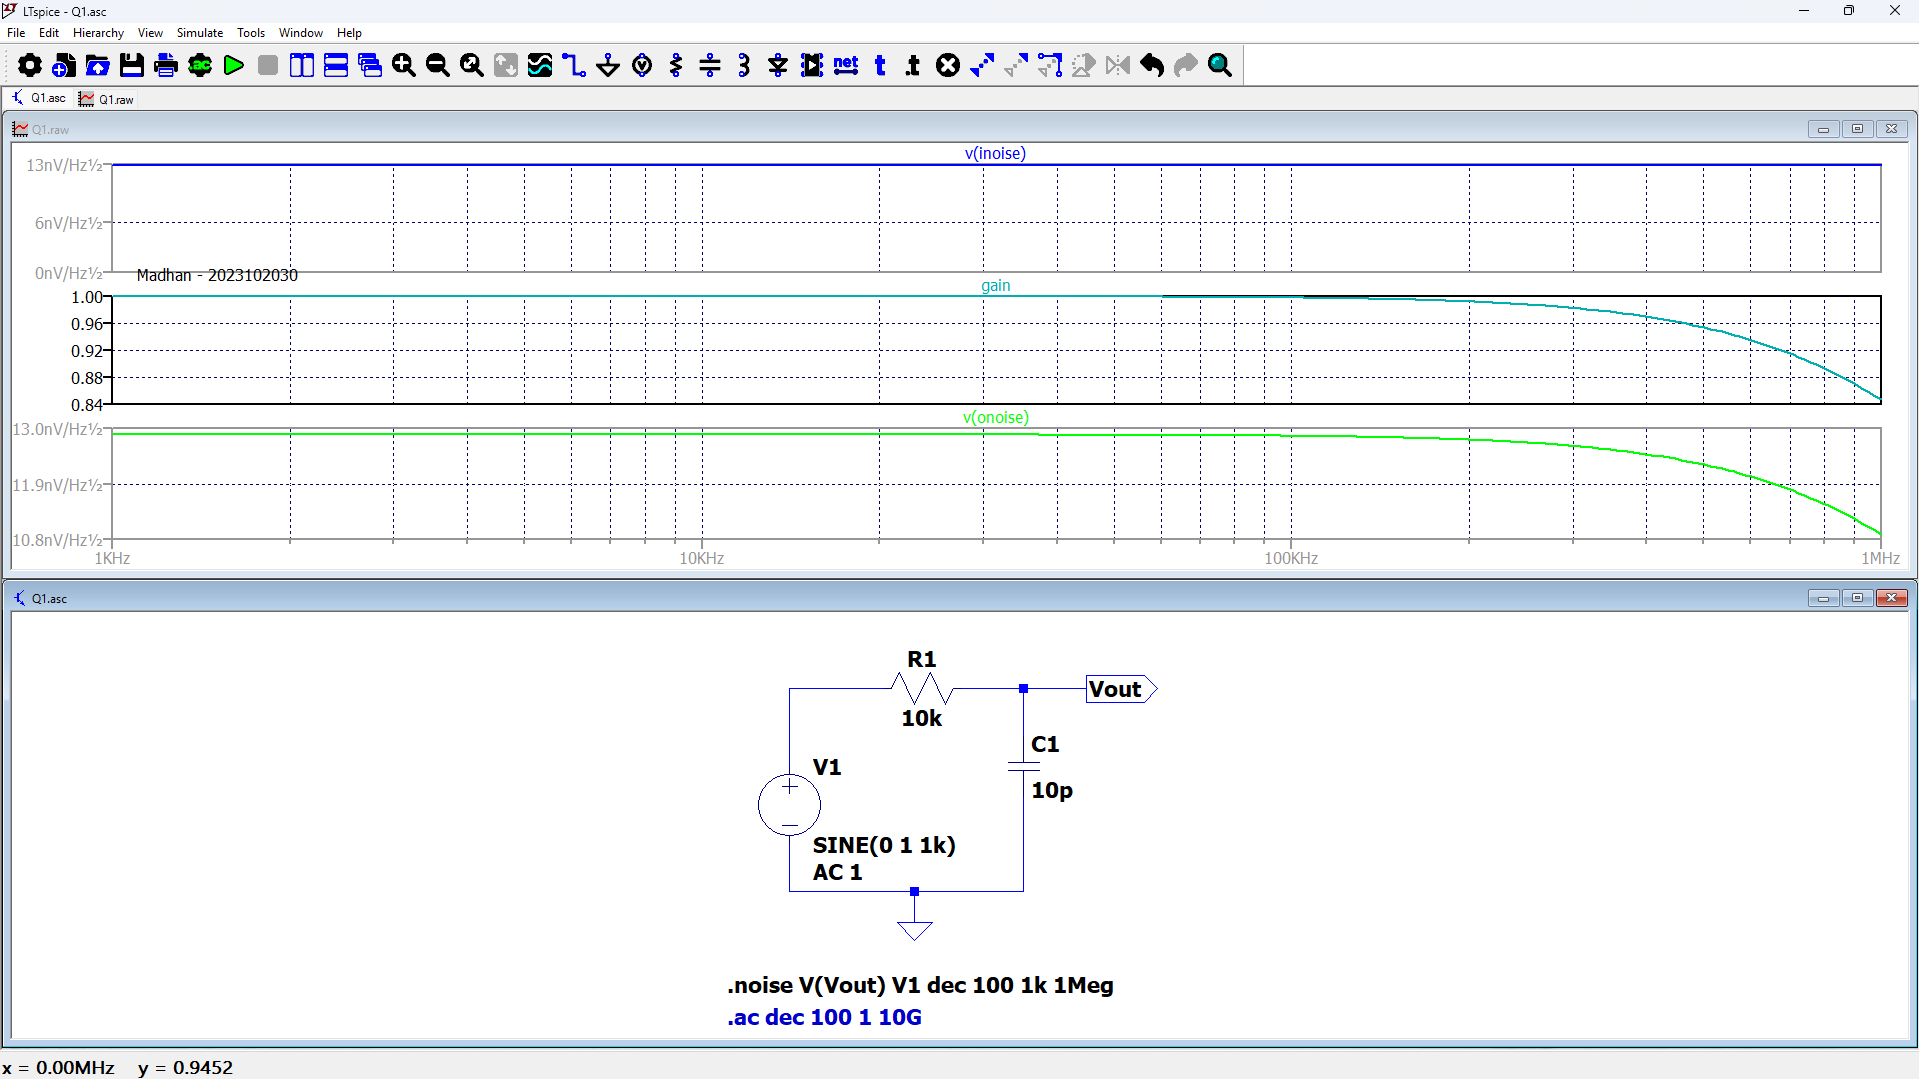
\includegraphics[width=0.8\textwidth]{images/q2_c.png}
    \caption{AC gain magnitude, output noise spectrum, and input noise spectrum.}
\end{figure}
\begin{figure}[H]
    \centering
    
\includegraphics[width=0.8\textwidth]{images/q2_c_2.png}
    \caption{AC gain magnitude, output noise spectrum, and input noise spectrum for the second bandwidth case.}
\end{figure}
\textit{Verification:} The plotted spectral density curves clearly demonstrate the relationship $v_{n_{out}}^2 = A_v^2 \times v_{n_{in}}^2$. The input white noise floor is shaped exactly by the first-order low-pass filter's transfer function $\left|A_v\right|^2$, confirming the theoretical basis.


\subsection*{(d) $R = 20 \text{ k}\Omega$ and $C = 10 \text{ pF}$ Case}
\textbf{Calculated $v_{n_{out}}$:} Assuming infinite bandwidth as in Part (a) Case 1, the total integrated noise depends only on the capacitor:
\begin{equation}
    P_{n_{out}} = \frac{kT}{C} = \frac{4.142 \times 10^{-21}}{10 \times 10^{-12}} = 4.142 \times 10^{-10} \text{ V}^2 \implies \mathbf{v_{n_{out}} = 20.35 \text{ } \mu\text{V}}
\end{equation}

\begin{figure}[H]
    \centering
    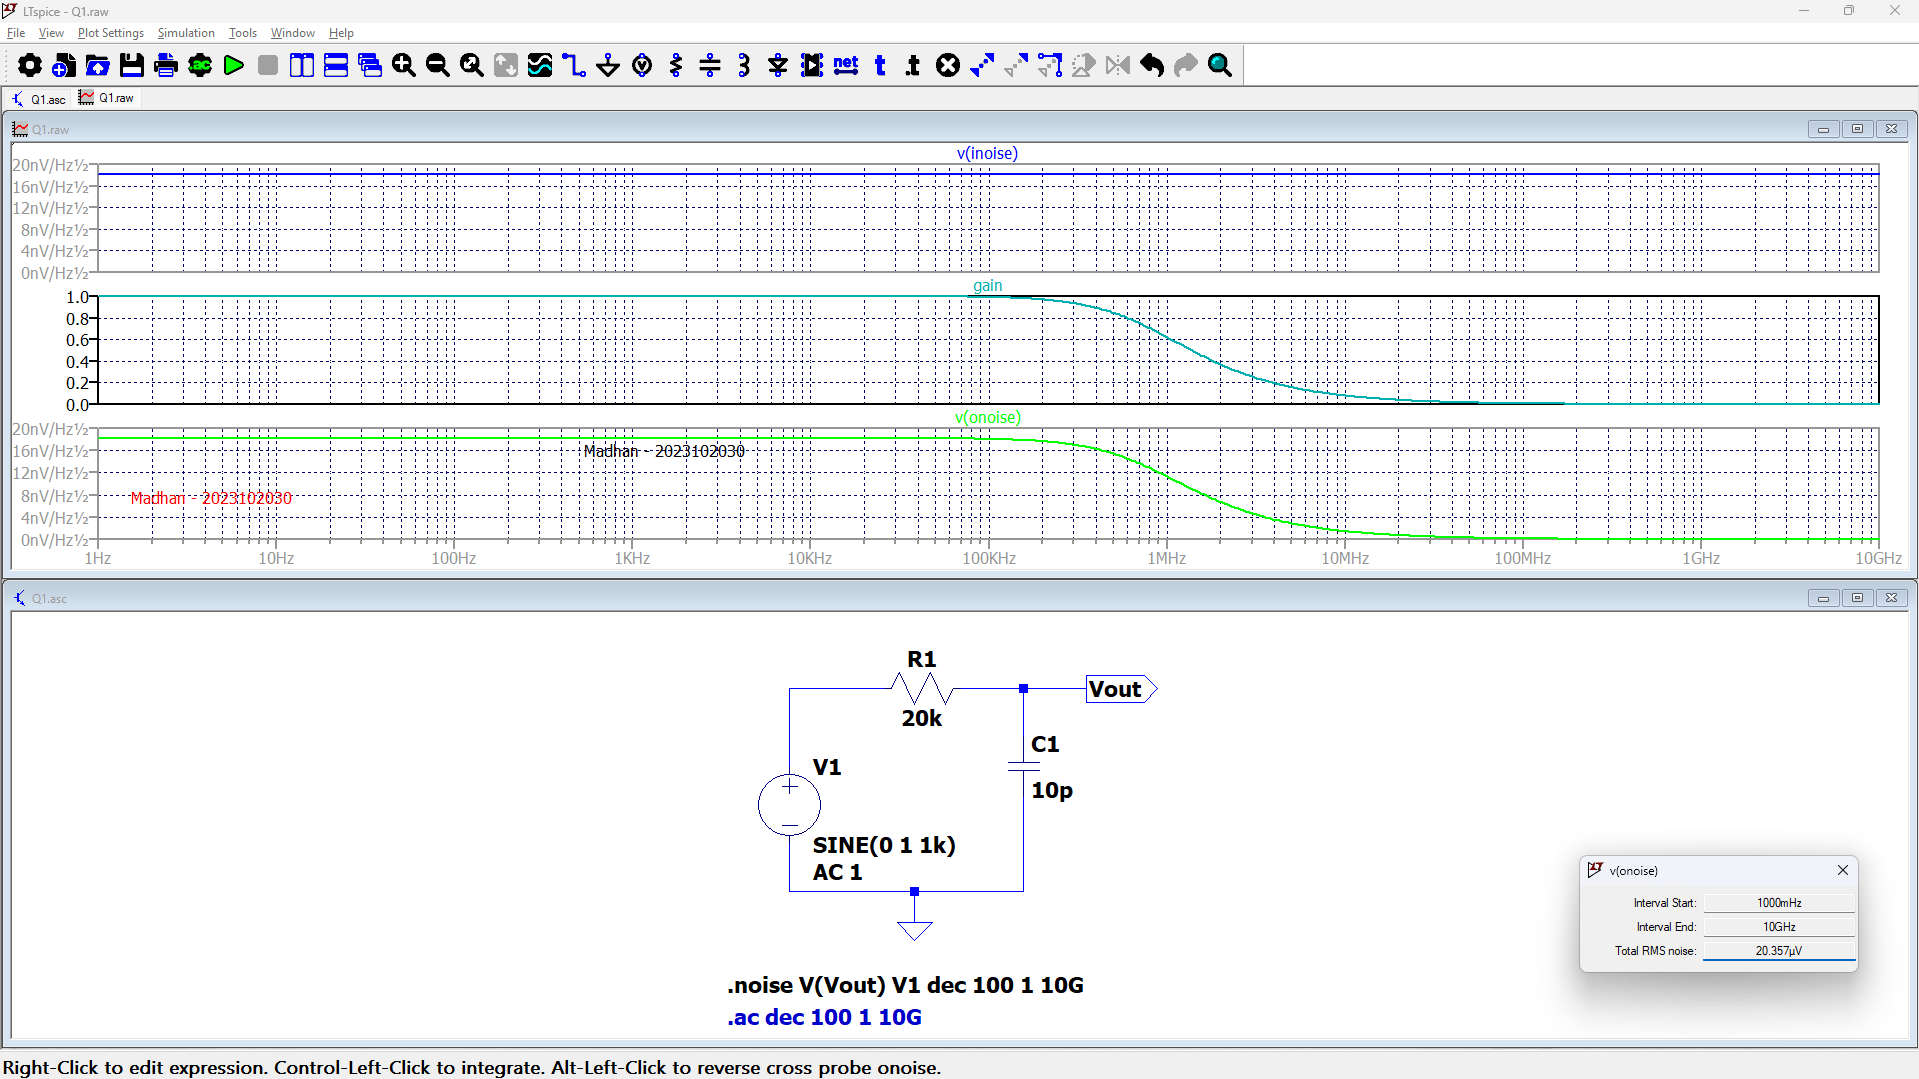
\includegraphics[width=0.8\textwidth]{images/q2_d.png}
    \caption{Gain and noise plots for $R = 20 \text{ k}\Omega, C = 10 \text{ pF}$.}
\end{figure}
\textit{Comparison \& Comments:} Even though the resistor value doubled (which increases the noise spectral density $4kTR$), the RC time constant also doubled, cutting the bandwidth of the filter in half. The increase in the noise floor is perfectly canceled out by the reduction in bandwidth. Therefore, the total integrated noise voltage remains constant at $20.35\,\mu\text{V}$.


\subsection*{(e) $R = 10 \text{ k}\Omega$ and $C = 20 \text{ pF}$ Case}
\textbf{Calculated $v_{n_{out}}$:}
\begin{equation}
    P_{n_{out}} = \frac{kT}{C} = \frac{4.142 \times 10^{-21}}{20 \times 10^{-12}} = 2.071 \times 10^{-10} \text{ V}^2 \implies \mathbf{v_{n_{out}} = 14.39 \text{ } \mu\text{V}}
\end{equation}

\begin{figure}[H]
    \centering
    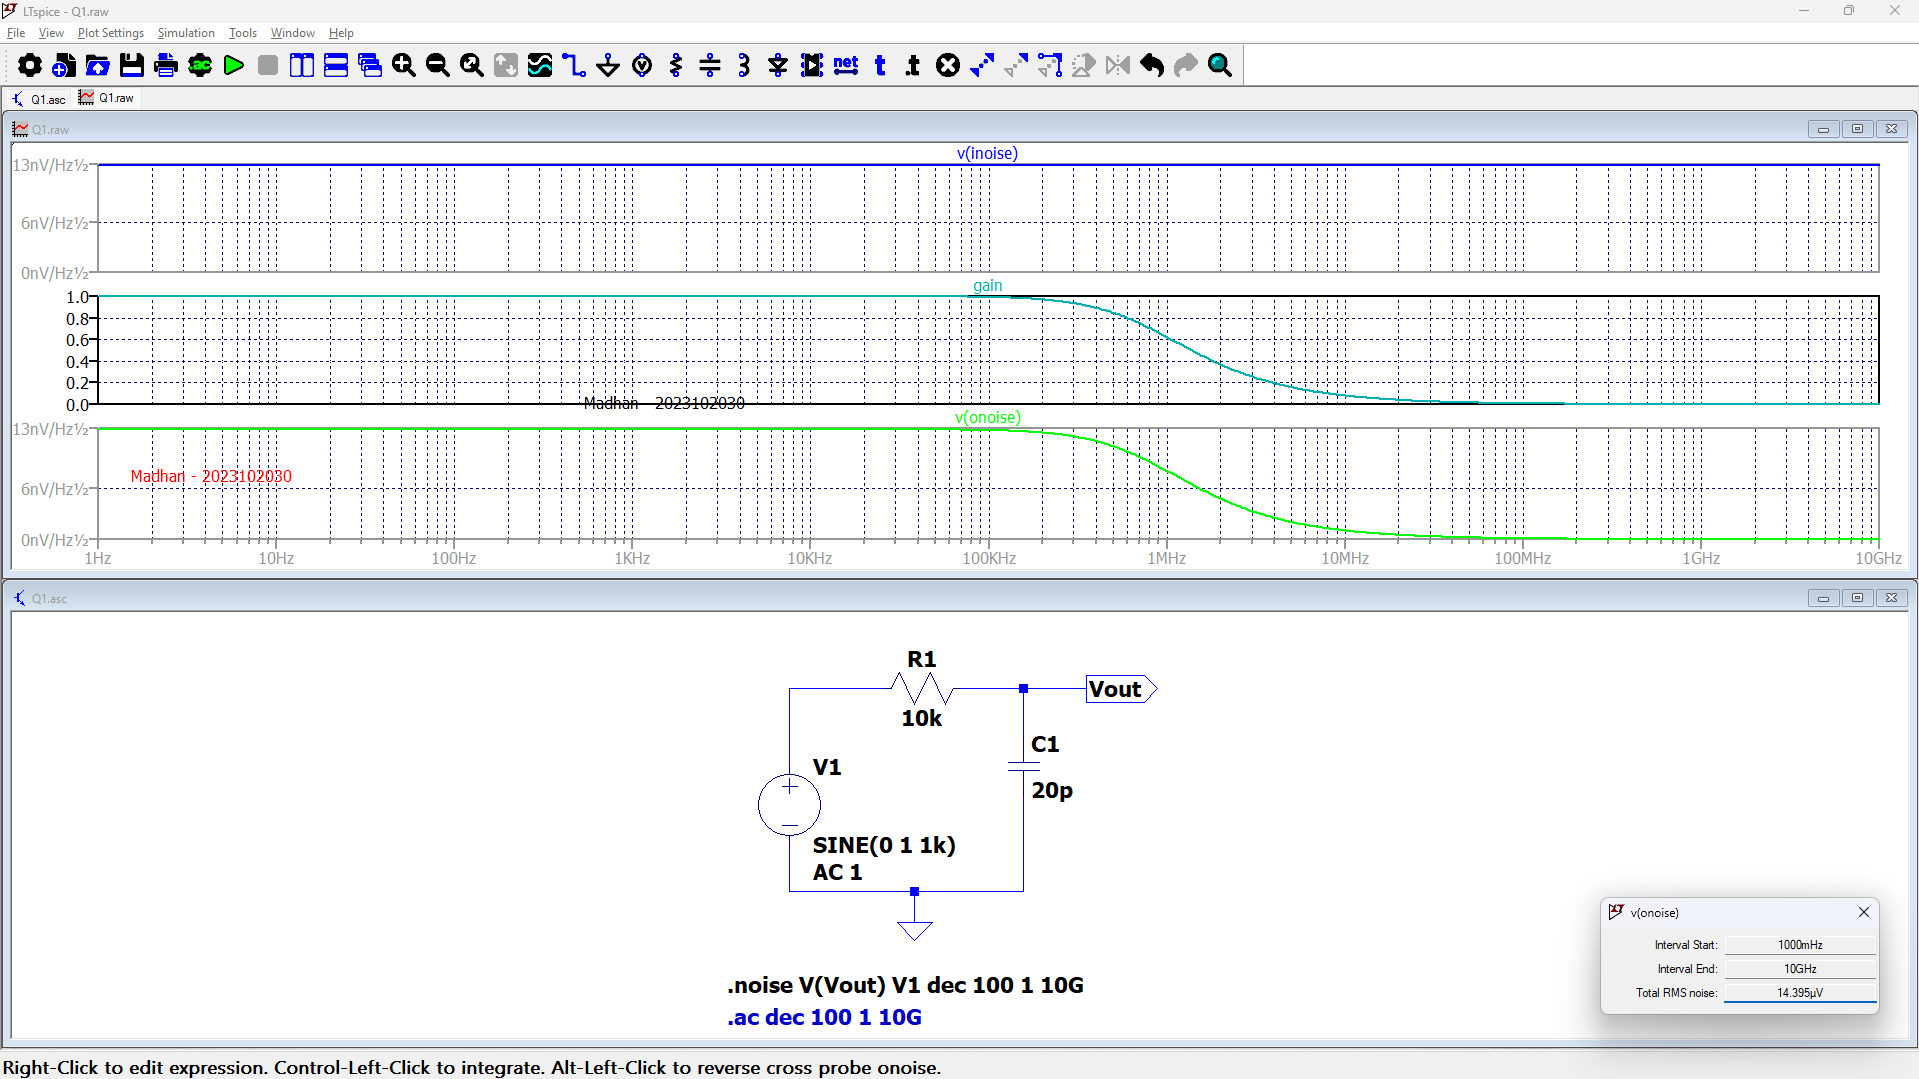
\includegraphics[width=0.8\textwidth]{images/q2_e.png}
    \caption{Gain and noise plots for $R = 10 \text{ k}\Omega, C = 20 \text{ pF}$.}
\end{figure}
\textit{Comparison \& Comments:} Increasing the capacitance directly reduces the total integrated noise power. Doubling the capacitance halves the total noise power ($P_{n_{out}}$), which results in a reduction of the rms noise voltage ($v_{n_{out}}$) by a factor of $\sqrt{2}$. This demonstrates the fundamental trade-off: to reduce $kT/C$ noise by half, the capacitor size must be quadrupled, costing significant area.

\newpage
% ==========================================
% QUESTION 3: Common Source Amplifier
% ==========================================
\section*{3. Common Source Amplifier with Drain Feedback Biasing}

\subsection*{(a) Derivation of Noise Expressions}
Assuming $R_B$ and $C_B$ are noiseless, the total noise is contributed by $M_1$. The drain noise current of $M_1$ includes thermal and flicker components:
\begin{equation}
    i_{n,M1}^2 = 4kT\gamma g_m + \frac{K}{C_{ox}WLf}g_m^2
\end{equation}
Since $C_B = 1\text{ F}$, it acts as an AC short. When $V_{in}$ is grounded for output noise analysis, the gate is at AC ground. $R_B$ effectively appears in parallel with $r_o$. The output noise voltage is:
\begin{equation}
    v_{n_{out}}^2 = i_{n,M1}^2 \times (r_o \parallel R_B)^2 = \left( 4kT\gamma g_m + \frac{K}{C_{ox}WLf}g_m^2 \right) (r_o \parallel R_B)^2
\end{equation}
The input-referred noise is the output noise divided by the squared gain ($A_v = g_m (r_o \parallel R_B)$):
\begin{equation}
    v_{n_{in}}^2 = \frac{v_{n_{out}}^2}{A_v^2} = \frac{v_{n_{out}}^2}{g_m^2 (r_o \parallel R_B)^2} = \frac{4kT\gamma}{g_m} + \frac{K}{C_{ox}WLf}
\end{equation}

\subsection*{(b) Simulation Analysis ($W/L = 0.36\mu/0.18\mu$)}
\begin{figure}[H]
    \centering
    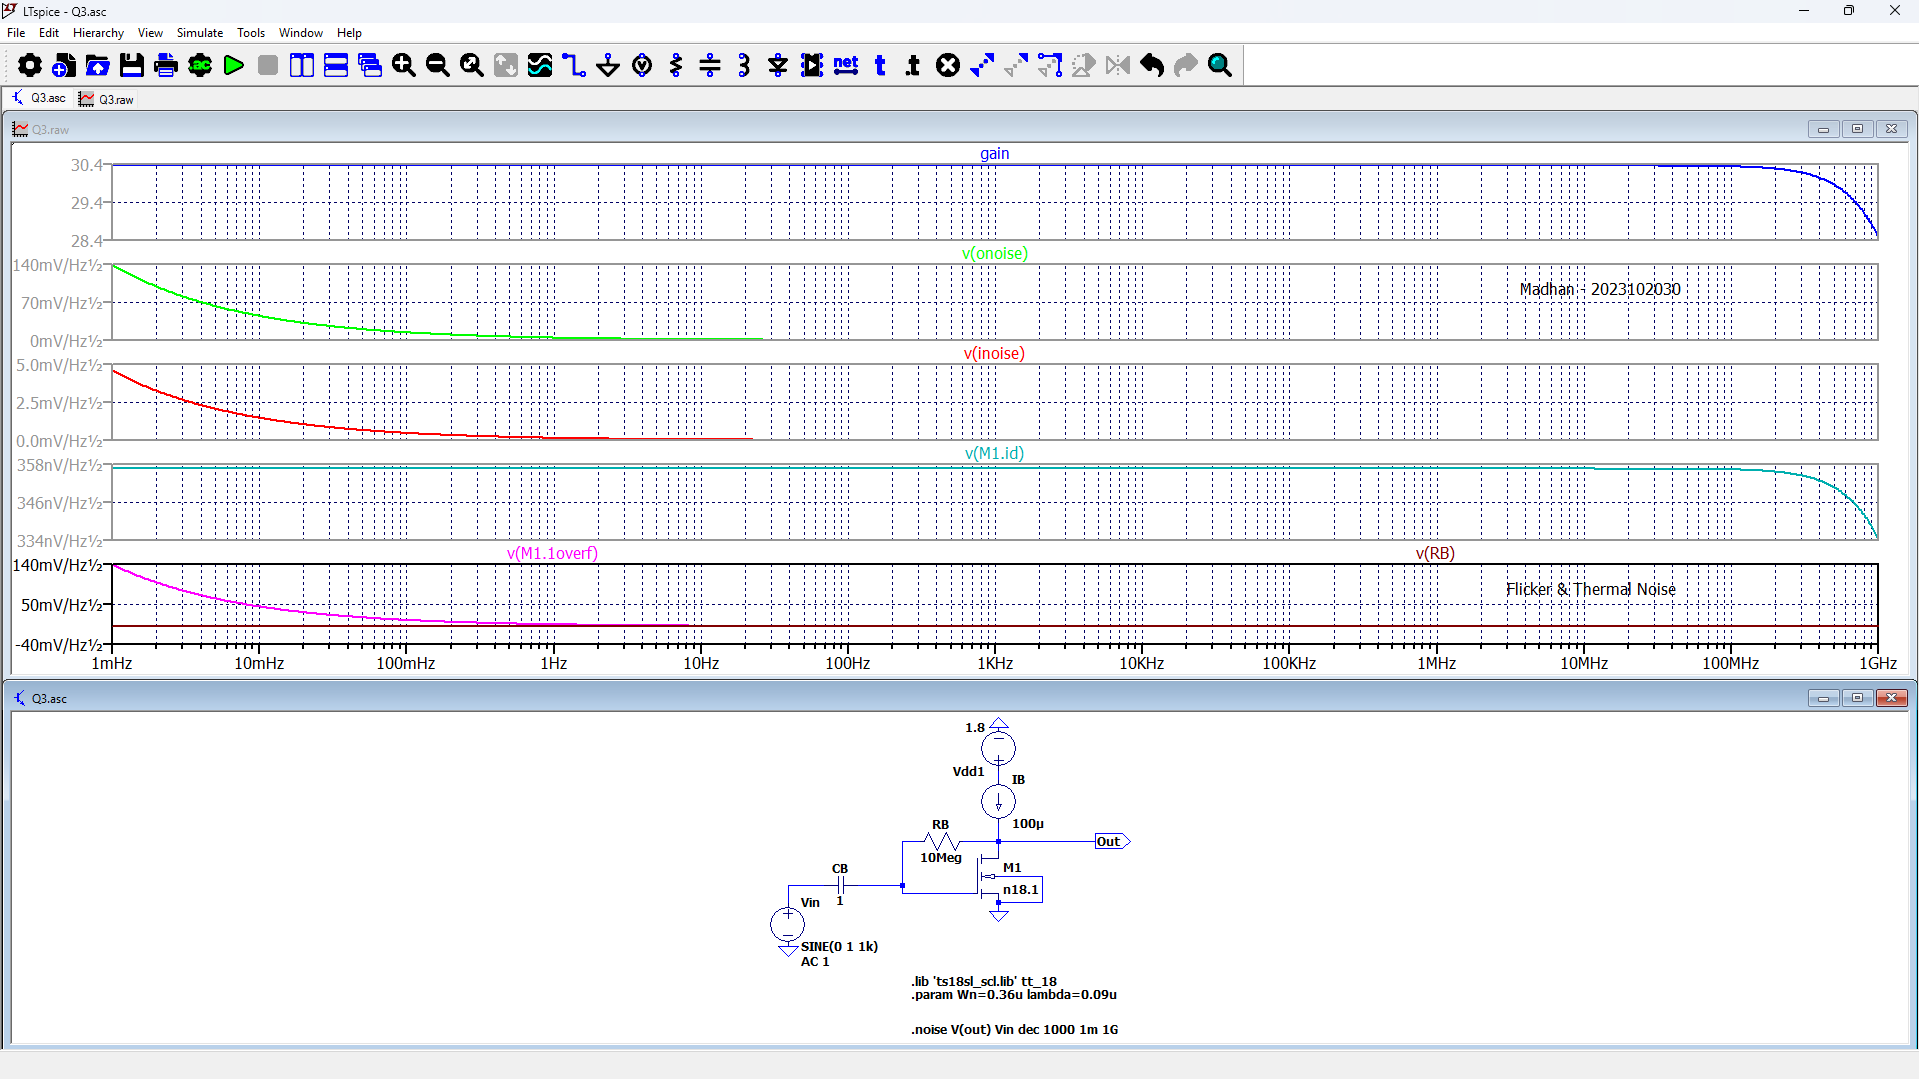
\includegraphics[width=0.8\textwidth]{images/q3_b.png}
    \caption{Gain, output noise, input referred noise, thermal noise, and flicker noise for $L=0.18\mu$.}
\end{figure}
\textit{Verification:} The plots verify that across the spectrum, $v_{n_{out}}$ is consistently equal to $A_v \times v_{n_{in}}$ when measured at any given frequency, confirming the theoretical scaling.

\subsection*{(c) Exact Estimation of $g_m$ and $r_o$}

\textbf{1. Transconductance ($g_m$):} \\
At high frequencies, the $1/f$ noise is negligible, and the input-referred noise floor is dominated by the thermal noise of $M_1$. The input-referred thermal noise spectral density is:
\begin{equation}
    v_{n_{in,th}}^2 \approx \frac{4kT\gamma}{g_m}
\end{equation}
Assuming the channel noise factor $\gamma \approx 2/3$ and $T=300\text{ K}$, we can rearrange the equation to solve for $g_m$:
\begin{equation}
    g_m = \frac{8kT/3}{(v_{n_{in,th}})^2}
\end{equation}
From the high-frequency flat band of our simulated noise plot, we observe $v_{n_{in,th}} = 12.991 \text{ nV}/\sqrt{\text{Hz}}$. Substituting this value:
\begin{equation}
    g_m \approx \frac{1.104 \times 10^{-20}}{(12.991 \times 10^{-9})^2} \approx \mathbf{65.41 \ \mu\text{S}}
\end{equation}

\vspace{0.5cm}
\textbf{2. Output Resistance ($r_o$):} \\
To extract $r_o$ accurately, we apply exact nodal analysis to account for signal feedforward through $R_B$. Assuming $C_B$ is an AC short, $v_{g} = v_{in}$. Applying KCL at the output node ($v_{out}$):
\begin{equation}
    \frac{v_{out}}{r_o} + \frac{v_{out} - v_{in}}{R_B} + g_m v_{in} = 0
\end{equation}
Grouping the terms and solving for the exact voltage gain $A_v$:
\begin{equation}
    v_{out} \left( \frac{1}{r_o} + \frac{1}{R_B} \right) = -v_{in} \left( g_m - \frac{1}{R_B} \right) \implies A_v = -\frac{g_m - \frac{1}{R_B}}{\frac{1}{r_o} + \frac{1}{R_B}}
\end{equation}
Using the magnitude of the mid-band gain $|A_v|$ and isolating $r_o$, we obtain our exact extraction formula:
\begin{equation}
    \frac{1}{r_o} + \frac{1}{R_B} = \frac{g_m - \frac{1}{R_B}}{|A_v|} \implies r_o = \left( \frac{g_m - \frac{1}{R_B}}{|A_v|} - \frac{1}{R_B} \right)^{-1}
\end{equation}
From the AC simulation, the linear mid-band gain is $|A_v| = 30.36$. Substituting our extracted $g_m$ and $1/R_B = 10^{-7} \text{ S}$:
\begin{equation}
    r_o = \left( \frac{65.41\mu - 0.1\mu}{30.36} - 0.1\mu \right)^{-1} = \left( 2.151\mu - 0.1\mu \right)^{-1} \approx \mathbf{487.5 \text{ k}\Omega}
\end{equation}

\subsection*{(d) Corner Frequency ($f_c$)}
\begin{figure}[H]
    \centering
    
\includegraphics[width=0.8\textwidth]{images/q3_d.png}
    \caption{Simulation plots showing the intersection of $1/f$ noise and thermal noise floor to determine $f_c$.}
\end{figure}
From the simulation plots, the frequency where the $1/f$ noise curve intersects the thermal noise floor is:
$f_c \approx$ \textbf{219.2216MHz}

\subsection*{(e) Case: $W/L = 2\mu/1\mu$}

\textbf{Simulation Results \& Comparison:} \\
For the scaled-up transistor design ($W/L = 2\mu/1\mu$), the corner frequency is extracted as:
\begin{equation}
    f_c \approx 4.60 \text{ MHz}
\end{equation}

\begin{figure}[H]
    \centering
    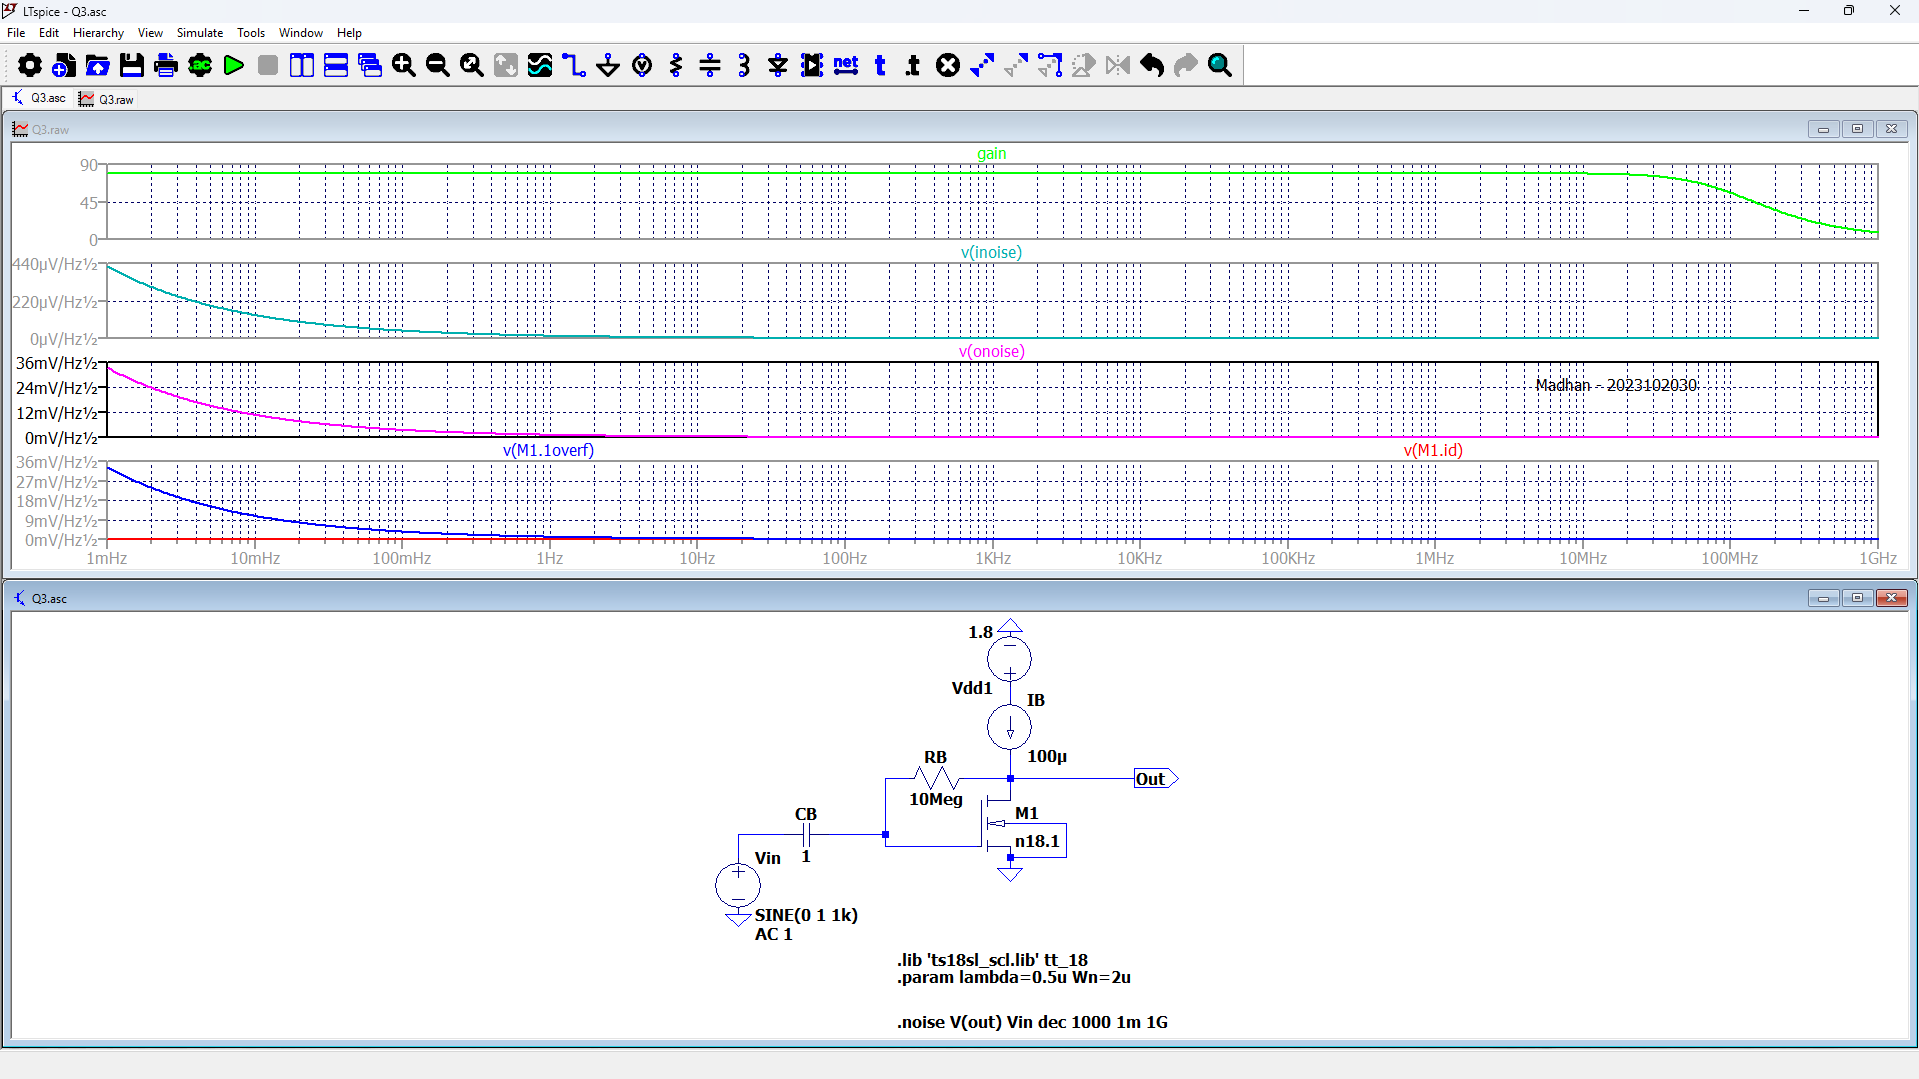
\includegraphics[width=0.8\textwidth]{images/q3_e.png}
    \caption{Simulation plots for $W/L = 2\mu/1\mu$ showing AC gain and Noise PSD.}
\end{figure}

Comparing this to the initial baseline design ($W/L = 0.36\mu/0.18\mu$):
\begin{itemize}
    \item \textbf{Total Input-Referred Noise ($v_{n_{in,Total}}$):} Decreased from $918.64 \ \mu\text{V}$ to $242.22 \ \mu\text{V}$.
    \item \textbf{Total Output Noise ($v_{n_{out,Total}}$):} Decreased from $27.765 \text{ mV}$ to $9.053 \text{ mV}$.
    \item \textbf{Gain ($A_v$):} Increased from $30.36$ to $79.05$.
    \item \textbf{Flicker Noise Density (@ 1 kHz):} Dropped significantly from $152.99 \ \mu\text{V}/\sqrt{\text{Hz}}$ to $36.68 \ \mu\text{V}/\sqrt{\text{Hz}}$.
\end{itemize}

\vspace{0.3cm}
\textbf{Discussion on Noise Performance and Trade-offs:} \\
Although the aspect ratio ($W/L = 2$) and the bias current ($I_B = 100 \ \mu\text{A}$) remained constant between the two cases, the physical gate area ($W \times L$) increased from $0.0648 \ \mu\text{m}^2$ to $2.0 \ \mu\text{m}^2$ (roughly a $30\times$ increase). This scaling introduces key architectural impacts and trade-offs:
\begin{enumerate}
    \item \textbf{Flicker Noise Suppression:} Flicker ($1/f$) noise power is inversely proportional to the gate area ($\propto \frac{1}{WL}$). The massive increase in area drastically suppressed the $1/f$ noise. This is the primary reason the input-referred noise dropped by nearly 75\% and the corner frequency $f_c$ shifted heavily to a lower frequency (from $\approx 219 \text{ MHz}$ down to $4.6 \text{ MHz}$).
    \item \textbf{Gain Improvement:} The channel length $L$ was increased from $0.18\mu$ to $1\mu$. Because channel length modulation effects are reduced in longer devices, the small-signal output resistance increases ($r_o \propto L$). This higher $r_o$ drove the mid-band voltage gain up from $30.36$ to $79.05$.
    \item \textbf{The Design Trade-off (Area vs. Bandwidth):} The major trade-off for achieving lower low-frequency noise and higher gain is a severe penalty in silicon area and high-frequency bandwidth. The larger gate area introduces significantly higher parasitic capacitances ($C_{gs}$ and $C_{gd}$). This increased capacitance heavily degrades the dominant pole frequency, thereby severely restricting the amplifier's $-3\text{ dB}$ bandwidth.
\end{enumerate}

\subsection*{(f) Case: $W/L = 4\mu/2\mu$}

\textbf{Simulation Results \& Comparison:} \\
For the largest transistor design ($W/L = 4\mu/2\mu$), the corner frequency is extracted as:
\begin{equation}
    f_c \approx 1.08 \text{ MHz}
\end{equation}

\begin{figure}[H]
    \centering
    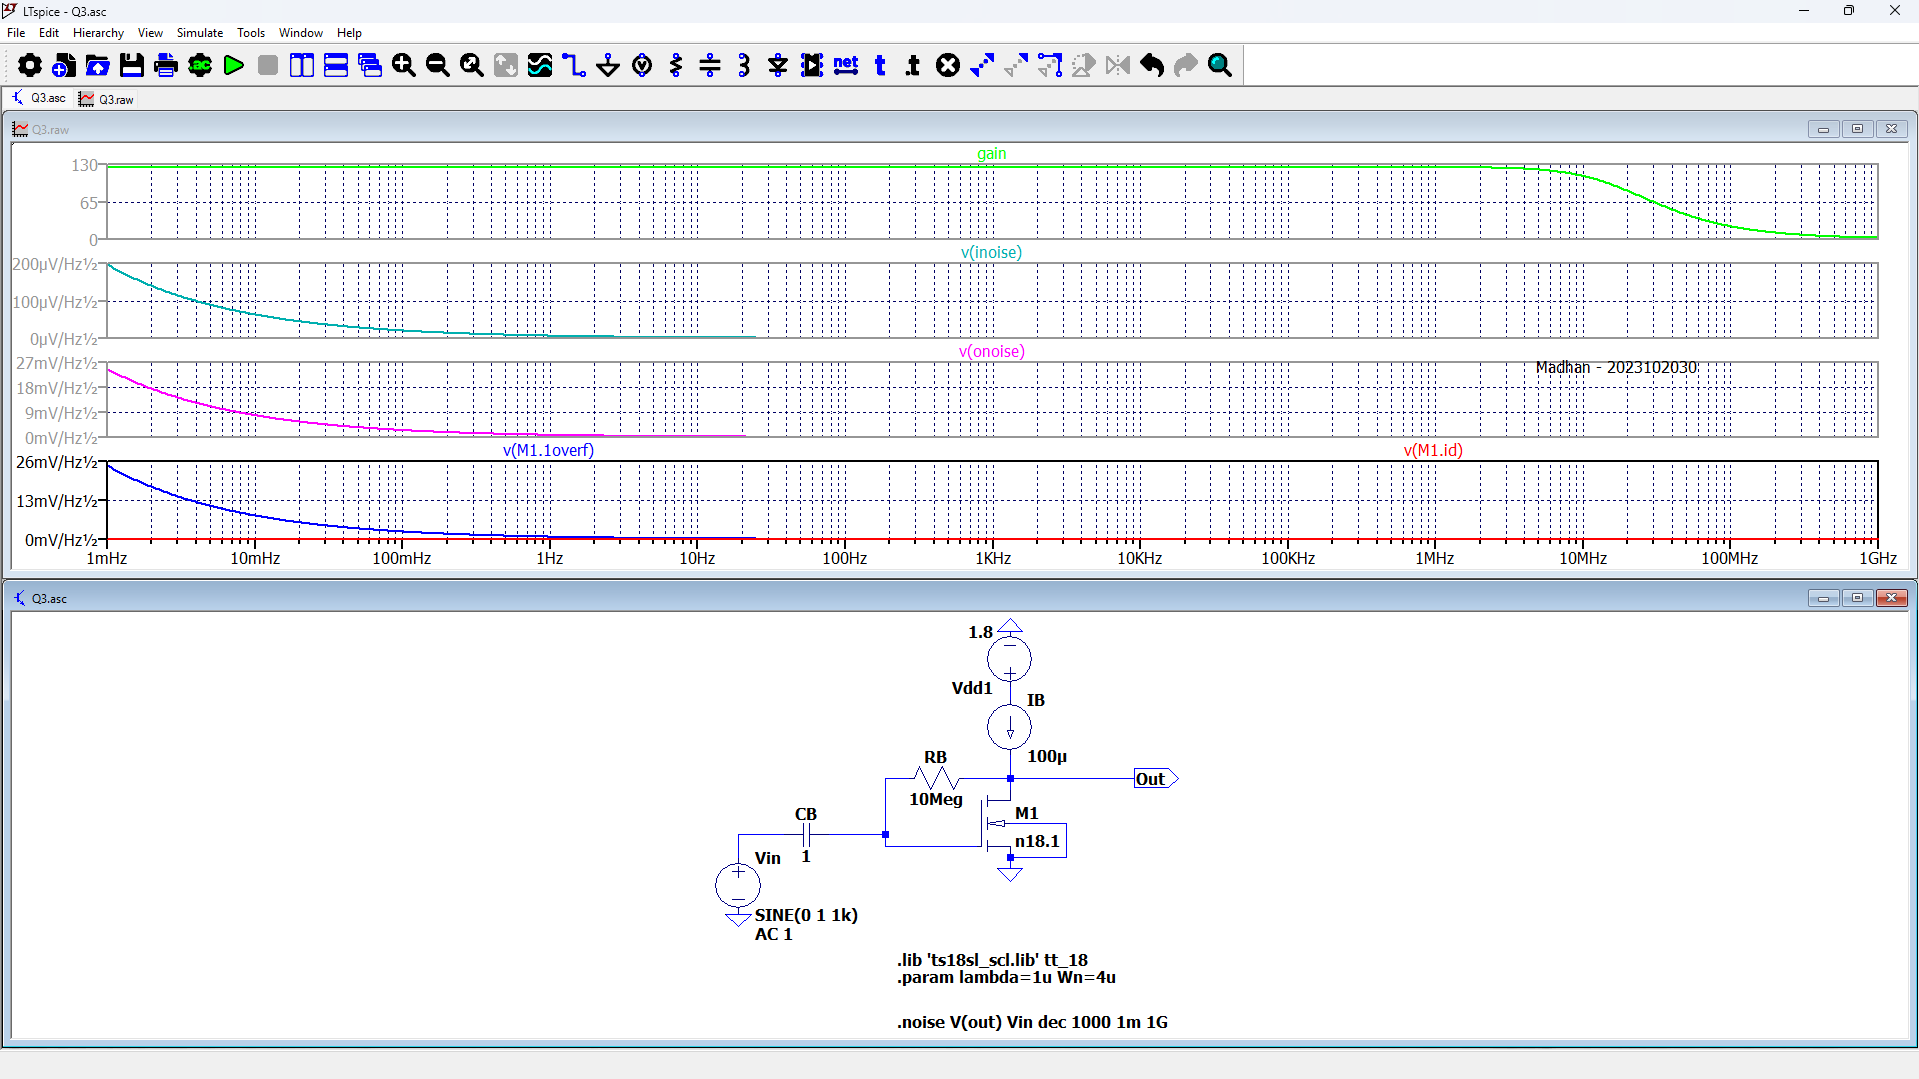
\includegraphics[width=0.8\textwidth]{images/q3_f.png}
    \caption{Simulation plots for $W/L = 4\mu/2\mu$ showing AC gain and Noise PSD.}
\end{figure}

Comparing this to the intermediate design ($W/L = 2\mu/1\mu$):
\begin{itemize}
    \item \textbf{Total Input-Referred Noise ($v_{n_{in,Total}}$):} Decreased from $242.22 \ \mu\text{V}$ to $212.54 \ \mu\text{V}$.
    \item \textbf{Total Output Noise ($v_{n_{out,Total}}$):} Decreased from $9.05 \text{ mV}$ to $6.16 \text{ mV}$.
    \item \textbf{Gain ($A_v$):} Increased significantly from $79.05$ to $125.04$.
    \item \textbf{Flicker Noise Density (@ 1 kHz):} Dropped from $36.68 \ \mu\text{V}/\sqrt{\text{Hz}}$ to $27.01 \ \mu\text{V}/\sqrt{\text{Hz}}$.
\end{itemize}

\vspace{0.3cm}
\textbf{Discussion on Noise Performance and Trade-offs:} \\
By continuing to scale up both the width and length by a factor of 2 (maintaining the aspect ratio $W/L = 2$), the gate area ($W \times L$) quadrupled from $2.0 \ \mu\text{m}^2$ to $8.0 \ \mu\text{m}^2$.
\begin{enumerate}
    \item \textbf{Diminishing Returns on Noise Reduction:} The $1/f$ noise density continued to drop, pushing the corner frequency $f_c$ down to $1.08 \text{ MHz}$. However, the relative improvement in total input-referred noise is less drastic than the first scaling step. This indicates that as area scales up, $1/f$ noise is heavily suppressed, leaving the constant thermal noise floor as the dominant contributor to the integrated noise.
    \item \textbf{Continuous Gain Increase:} Because the channel length $L$ doubled to $2\mu$, the small-signal output resistance $r_o$ increased proportionally. This pushed the mid-band voltage gain up to $125.04$.
    \item \textbf{The Extreme Trade-off:} While this design yields the highest gain and lowest low-frequency noise, it represents an extreme architectural trade-off. An $8.0 \ \mu\text{m}^2$ gate area creates massive parasitic gate capacitances ($C_{gs}$ and $C_{gd}$). In practical design, this limits the amplifier to very low-frequency applications (such as low-speed sensor interfaces) due to severe bandwidth degradation.
\end{enumerate}

\subsection*{(g) Comparison Summary}

\begin{table}[H]
    \centering
    \caption{Noise Performance Comparison for Scaled Device Geometries}
    \renewcommand{\arraystretch}{1.3}
    \resizebox{\textwidth}{!}{
    \begin{tabular}{@{}cccccc@{}}
        \toprule
        \textbf{W/L} & \textbf{Gain (V/V)} & \textbf{1/f @ 1kHz ($\mu\text{V}/\sqrt{\text{Hz}}$)} & \textbf{$f_c$ (MHz)} & \textbf{$v_{n_{out,Total}}$ (mV)} & \textbf{$v_{n_{in,Total}}$ ($\mu\text{V}$)} \\
        \midrule
        $0.36\mu / 0.18\mu$ & 30.36 & 152.99 & 219.22 & 27.765 & 918.64 \\
        $2\mu / 1\mu$       & 79.05 & 36.68  & 4.60   & 9.053  & 242.22 \\
        $4\mu / 2\mu$       & 125.04 & 27.01  & 1.08   & 6.161  & 212.54 \\
        \bottomrule
    \end{tabular}}
\end{table}

\vspace{0.3cm}
\textbf{Summary and Inference:} \\
The simulation data clearly demonstrates the fundamental trade-offs in analog CMOS sizing. As the transistor dimensions are scaled up while maintaining a constant aspect ratio ($W/L = 2$) and constant bias current ($I_B = 100\ \mu\text{A}$), the following trends are observed:
\begin{enumerate}
    \item \textbf{Gain Increases:} As the channel length ($L$) increases ($0.18\mu \to 1\mu \to 2\mu$), the channel length modulation effect diminishes. This increases the small-signal output resistance ($r_o$), which directly drives up the mid-band voltage gain from 30.36 to 125.04.
    \item \textbf{Flicker Noise Decreases:} Flicker ($1/f$) noise power is inversely proportional to the total gate area ($W \times L$). As the area increased from $0.0648\ \mu\text{m}^2$ to $8.0\ \mu\text{m}^2$, the $1/f$ spot noise at 1 kHz plummeted. Consequently, the corner frequency ($f_c$) shifted drastically to the left, from $\approx 219 \text{ MHz}$ down to just $\approx 1 \text{ MHz}$.
    \item \textbf{Integrated Noise Decreases:} Due to the massive suppression of the low-frequency $1/f$ noise, the total integrated input-referred noise dropped by over 75\%. Interestingly, despite the massive increase in voltage gain, the total output noise also decreased. This occurs because the larger gate area introduces significant parasitic capacitance ($C_{gs}$, $C_{gd}$), which severely degrades the amplifier's high-frequency bandwidth, effectively filtering out higher-frequency thermal noise. 
\end{enumerate}
In conclusion, scaling up device area significantly improves gain and low-frequency noise characteristics, but at the direct cost of silicon area and high-frequency bandwidth.
\newpage
% ==========================================
% QUESTION 4: Noise Efficiency Factor (NEF)
% ==========================================
\section*{4. Noise Efficiency Factor (NEF)}

\subsection*{(a) Interpretation of NEF}
A lower NEF is better. The Noise Efficiency Factor (NEF) measures the trade-off between noise, bandwidth, and power consumption relative to a theoretical ideal bipolar transistor (which has an NEF of 1). A lower value indicates that the amplifier requires less total current to achieve the desired noise performance and bandwidth, making it highly power-efficient.

\subsection*{(b) Derivation of $v_{n_{in,rms}}$ Expression}

To derive the complete input-referred noise, we must determine the transfer function of the intrinsic noise current ($i_{n,x}$) from each MOSFET to the output node. The intrinsic noise current PSD for any MOSFET is:
\begin{equation}
    S_{i,x}(f) = \underbrace{4kT\gamma g_{mx}}_{\text{Thermal}} + \underbrace{\frac{K_x}{C_{ox} W_x L_x f} g_{mx}^2}_{\text{Flicker}}
\end{equation}

\textbf{1. Transconductance and Sizing Relationships:}\\
Based on Fig. 3, $M_2$ and $M_4$ are identical PMOS devices $(N_2 W_2/L_2)$ sharing the same bias, so $g_{m2} = g_{m4}$. 
$M_1$ and $M_3$ are identical NMOS devices $(N_1 W_1/L_1)$ sharing the same DC gate bias (via $R_B$), so $g_{m1} = g_{m3}$. 
$M_0$ is sized $(W_1/L_1)$. Because $M_3$ is $N_1$ times wider than $M_0$ and carries $N_1$ times the current, its transconductance scales by $N_1$: $g_{m3} = g_{m1} = N_1 g_{m0}$.

\textbf{2. Output Noise Current Contributions ($S_{i,out}$):}\\
We map each noise source to the output node:
\begin{itemize}
    \item \textbf{$M_1$ \& $M_2$:} Inject directly into the output. Contributions: $S_{i1}$ and $S_{i2}$.
    \item \textbf{$M_4$:} Noise $i_{n4}$ creates a voltage $v_{g4} = i_{n4}/g_{m4}$, driving $M_2$ to produce $i_{out,4} = g_{m2}(i_{n4}/g_{m4}) = i_{n4}$. Contribution: $S_{i4} = S_{i2}$.
    \item \textbf{$M_3$:} Noise $i_{n3}$ pulls from $M_4$, mirroring to $M_2$ with a gain of 1. Contribution: $S_{i3} = S_{i1}$.
    \item \textbf{$M_0$:} Noise $i_{n0}$ creates a voltage $v_{g0} = i_{n0}/g_{m0}$. Because $C_B = 1\text{ F}$ acts as a perfect AC short to the ideal voltage source $v_{in}$, the gate of $M_1$ is AC grounded. Thus, $v_{g0}$ does not modulate $M_1$. However, it modulates $M_3$, producing $i_{d3} = g_{m3}(i_{n0}/g_{m0}) = N_1 i_{n0}$, which then mirrors to the output. Contribution: $N_1^2 S_{i0}$.
\end{itemize}

Summing these contributions yields the total output noise current PSD:
\begin{equation}
    S_{i,out}(f) = 2S_{i1} + 2S_{i2} + N_1^2 S_{i0}
\end{equation}

\textbf{3. Simplification using Symmetry:}\\
We can express $N_1^2 S_{i0}$ purely in terms of $S_{i1}$. Substituting $g_{m0} = g_{m1}/N_1$ into the thermal and flicker components of $M_0$:
\begin{align*}
    N_1^2 S_{i0} &= N_1^2 \left( 4kT\gamma_N \frac{g_{m1}}{N_1} + \frac{K_N}{C_{ox} W_1 L_1 f} \frac{g_{m1}^2}{N_1^2} \right) \\
                 &= N_1 \left( 4kT\gamma_N g_{m1} \right) + N_1 \left( \frac{K_N}{C_{ox} (N_1 W_1) L_1 f} g_{m1}^2 \right) = N_1 S_{i1}
\end{align*}
This elegantly simplifies the total output noise current PSD:
\begin{equation}
    S_{i,out}(f) = (2 + N_1)S_{i1}(f) + 2S_{i2}(f)
\end{equation}

\textbf{4. Final Input-Referred RMS Noise Expression:}\\
The input-referred noise PSD, $S_{v,in}(f)$, is $S_{i,out}(f) / g_{m1}^2$. 
\begin{equation}
    S_{v,in}(f) = (2+N_1) \left( \frac{4kT\gamma_N}{g_{m1}} + \frac{K_N}{C_{ox} (N_1 W_1) L_1 f} \right) + 2 \left( \frac{4kT\gamma_P g_{m2}}{g_{m1}^2} + \frac{K_P g_{m2}^2}{C_{ox} (N_2 W_2) L_2 g_{m1}^2 f} \right)
\end{equation}

To find the total RMS noise voltage ($v_{n_{in,rms}}$), we integrate $S_{v,in}(f)$ over the operational bandwidth from $f_L$ to $f_H$. The thermal terms integrate linearly with bandwidth ($BW = f_H - f_L$), and the flicker terms integrate logarithmically:
\begin{equation}
    v_{n_{in,rms}} = \sqrt{ \int_{f_L}^{f_H} S_{v,in}(f) df } 
\end{equation}
\begin{equation}
    v_{n_{in,rms}} = \sqrt{ \underbrace{ \left( \frac{4kT (2+N_1)\gamma_N}{g_{m1}} + \frac{8kT\gamma_P g_{m2}}{g_{m1}^2} \right) BW }_{\text{Total Integrated Thermal Noise}} + \underbrace{ \left( \frac{K_N (2+N_1)}{C_{ox} N_1 W_1 L_1} + \frac{2 K_P g_{m2}^2}{C_{ox} N_2 W_2 L_2 g_{m1}^2} \right) \ln\left(\frac{f_H}{f_L}\right) }_{\text{Total Integrated Flicker Noise}} }
\end{equation}

\subsection*{(c) Noise Contributions Calculation ($M_1$ and $M_2$ Only)}

As requested, we isolate the input-referred RMS noise contributed strictly by the main amplifier devices ($M_1$ and $M_2$). From the LTspice \texttt{.noise} simulation, the individual RMS noise voltage contributions at the output node are extracted. Since noise components are uncorrelated, their powers add. The total input-referred RMS noise due to $M_1$ and $M_2$ is calculated as:
\begin{equation}
    v_{n_{in,rms}}(M_1, M_2) = \frac{\sqrt{v_{m1.id}^2 + v_{m1.1/f}^2 + v_{m2.id}^2 + v_{m2.1/f}^2}}{A_v}
\end{equation}

The extracted simulation data and the manually calculated $v_{n_{in,rms}}$ for the 1 Hz to 1 MHz bandwidth are tabulated below.

\begin{table}[H]
    \centering
    \caption{Noise Contributions for $M_1$ and $M_2$ (1 Hz to 1 MHz)}
    \renewcommand{\arraystretch}{1.4}
    \resizebox{\textwidth}{!}{
    \begin{tabular}{@{}ccccccccc@{}}
        \toprule
        \textbf{Case} & \textbf{$(W_1/L_1)$} & \textbf{$(W_2/L_2)$} & \textbf{m1.id} & \textbf{m1.loverf} & \textbf{m2.id} & \textbf{m2.loverf} & \textbf{Gain (V/V)} & \textbf{$v_{n_{in,rms}}$ (Calculated)} \\
        \midrule
        i   & $0.18\mu/0.18\mu$ & $0.18\mu/0.18\mu$ & $190.78\, \mu\text{V}$ & $3.954\, \text{mV}$ & $160.68\, \mu\text{V}$ & $3.496\, \text{mV}$ & $22.03$ & $\mathbf{239.86\, \mu\text{V}}$ \\
        ii  & $1\mu/1\mu$       & $1\mu/1\mu$       & $433.55\, \mu\text{V}$ & $1.694\, \text{mV}$ & $325.65\, \mu\text{V}$ & $2.014\, \text{mV}$ & $78.89$ & $\mathbf{34.06\, \mu\text{V}}$ \\
        iii & $10\mu/10\mu$     & $10\mu/10\mu$     & $801.90\, \mu\text{V}$ & $681.55\, \mu\text{V}$ & $591.09\, \mu\text{V}$ & $876.84\, \mu\text{V}$ & $336.97$ & $\mathbf{4.43\, \mu\text{V}}$ \\
        \bottomrule
    \end{tabular}}
\end{table}

\begin{figure}[H]
    \centering
    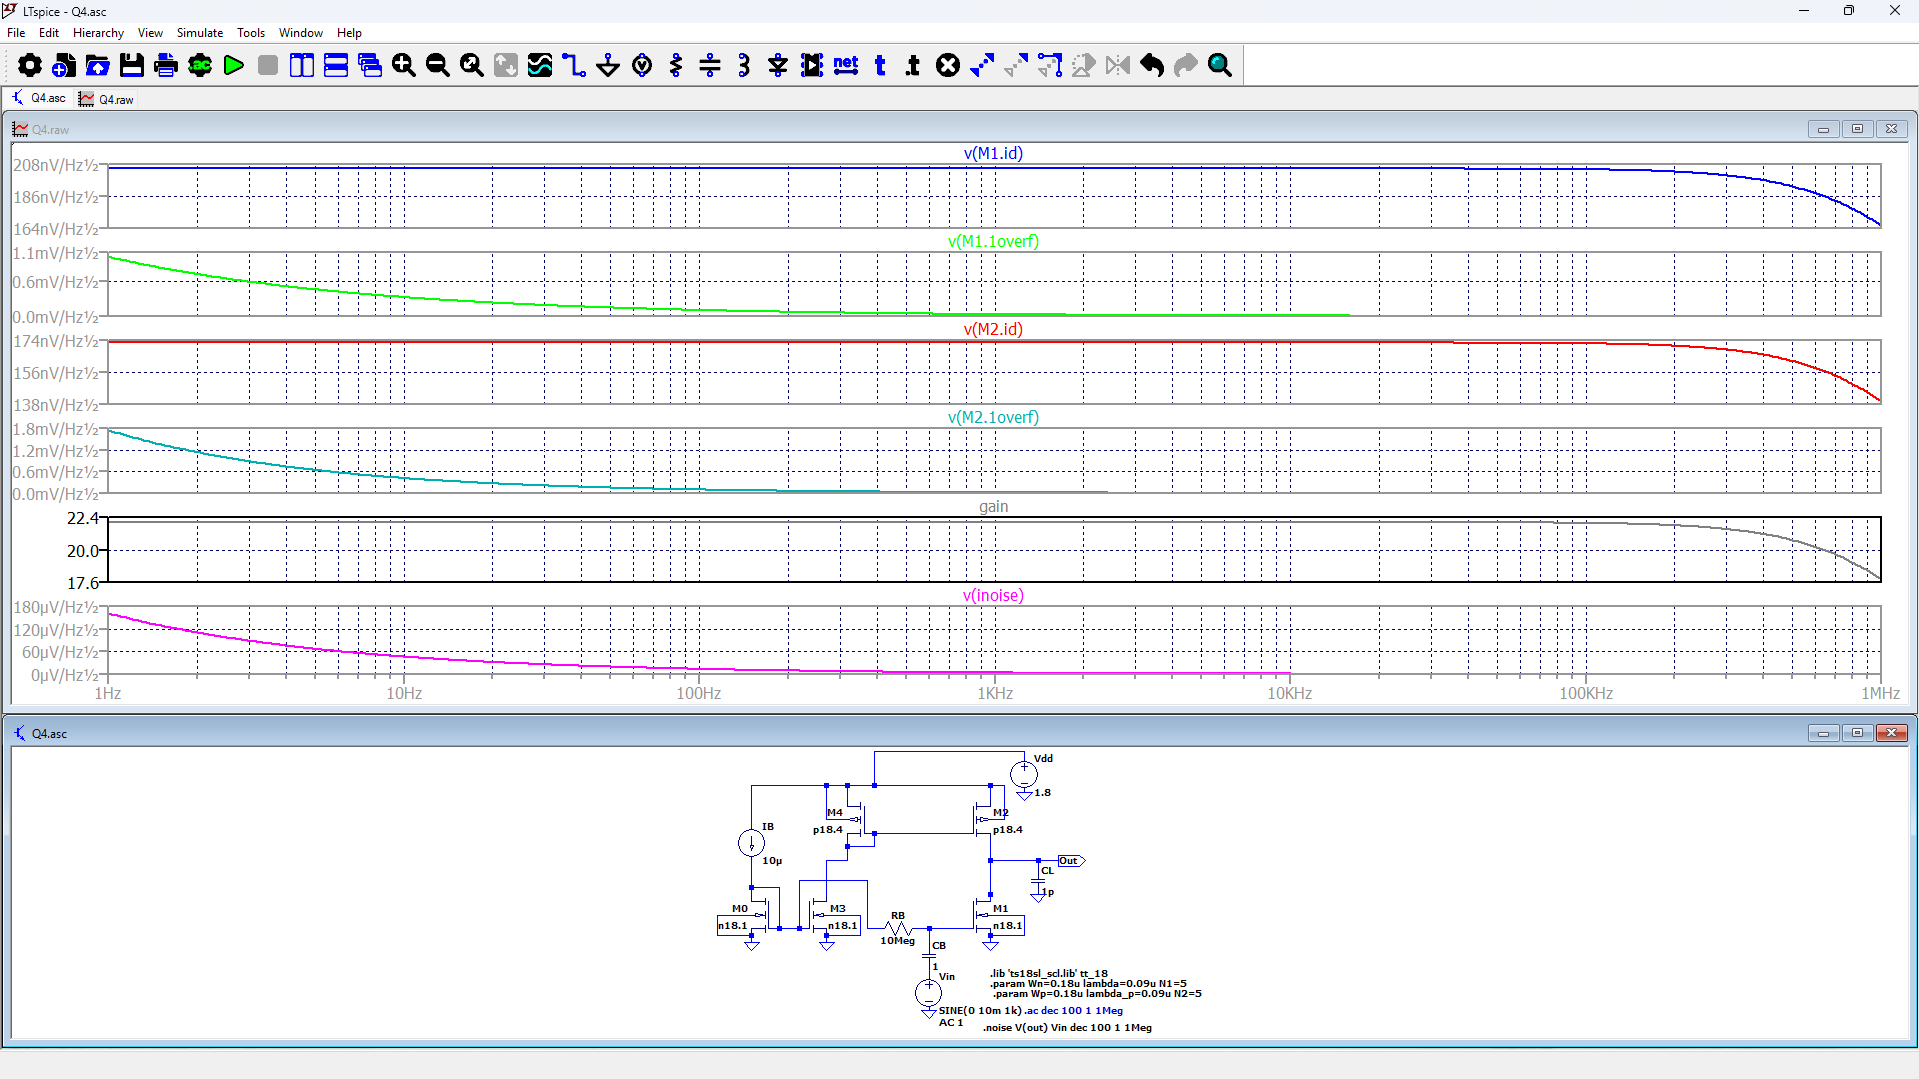
\includegraphics[width=0.9\textwidth]{images/q4_c_1.png}
    \caption{Simulation plots showing Noise PSD, Gain, and Bandwidth for the first case ($W/L = 0.18\mu/0.18\mu$).}
\end{figure}

\begin{figure}[H]
    \centering
    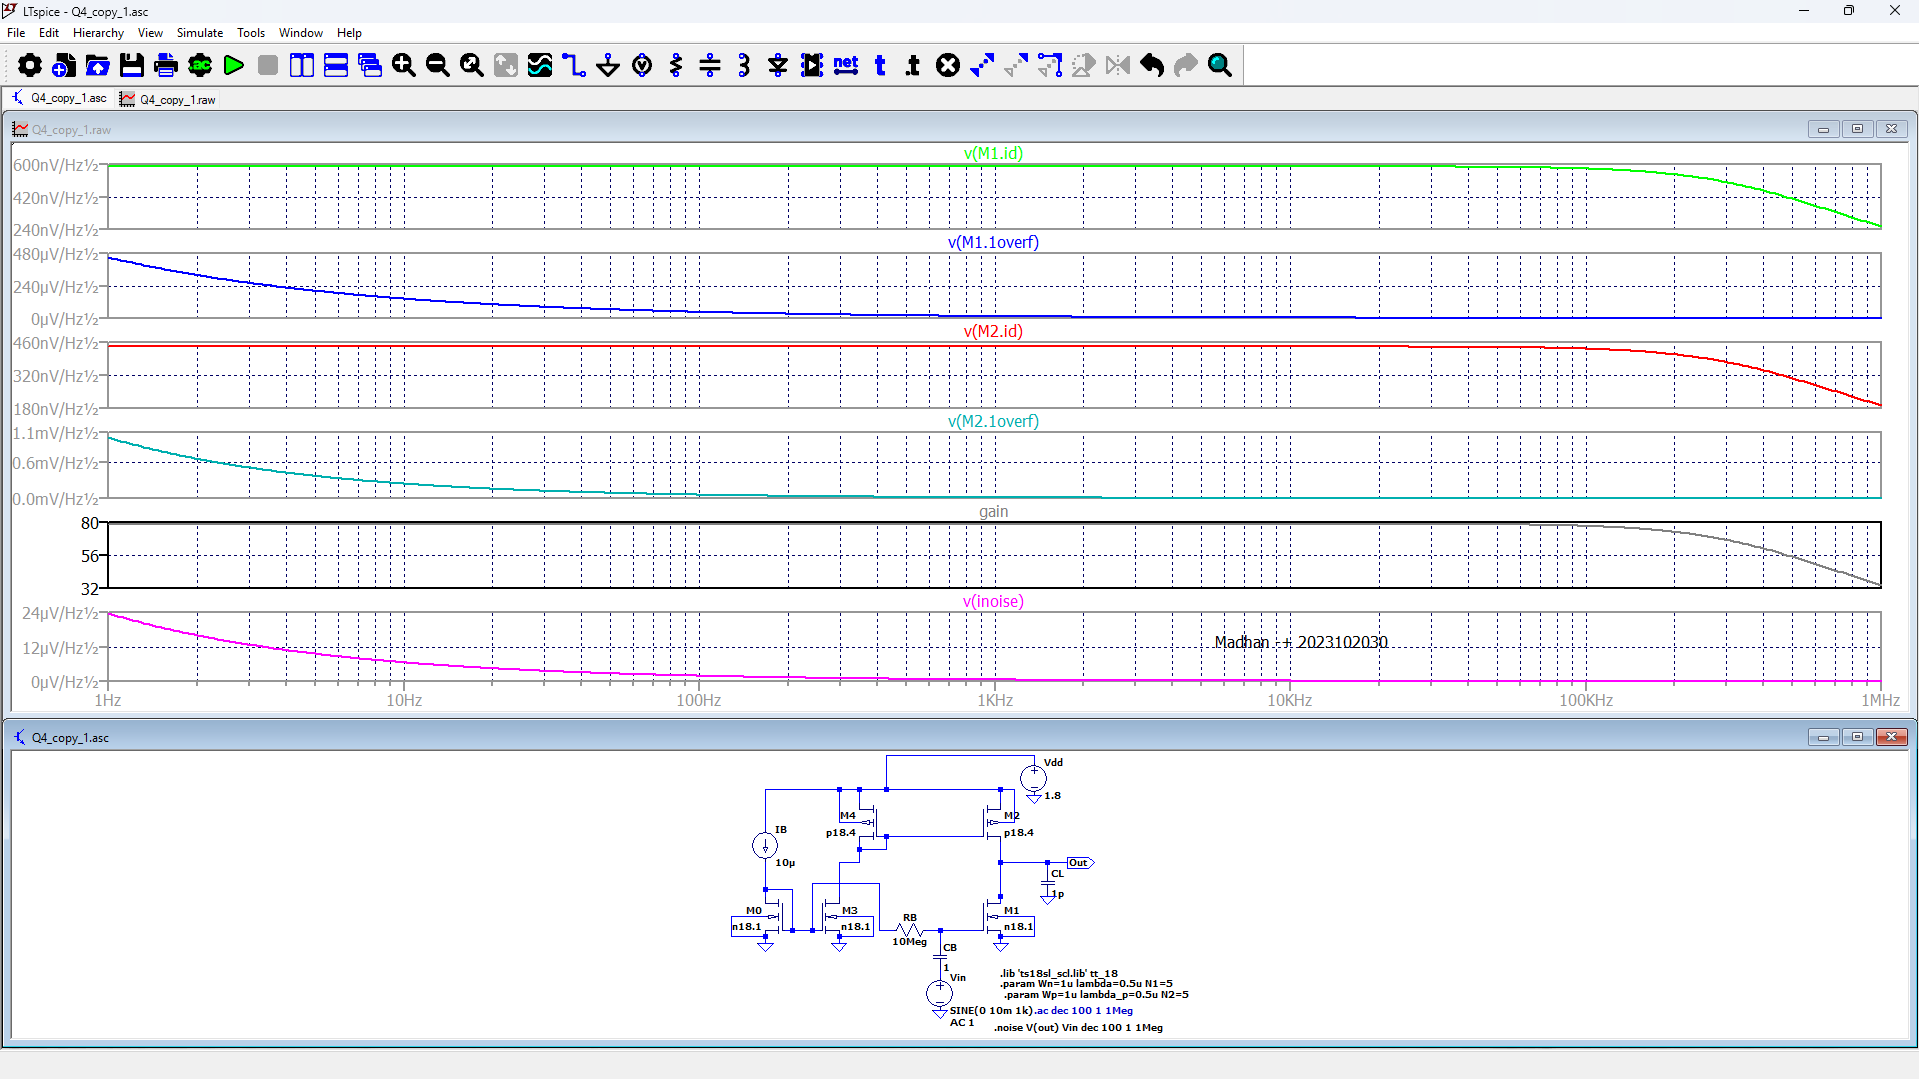
\includegraphics[width=0.9\textwidth]{images/q4_c_2.png}
    \caption{Simulation plots showing Noise PSD, Gain, and Bandwidth for the second case ($W/L = 1\mu/1\mu$).}
\end{figure}

\begin{figure}[H]
    \centering
    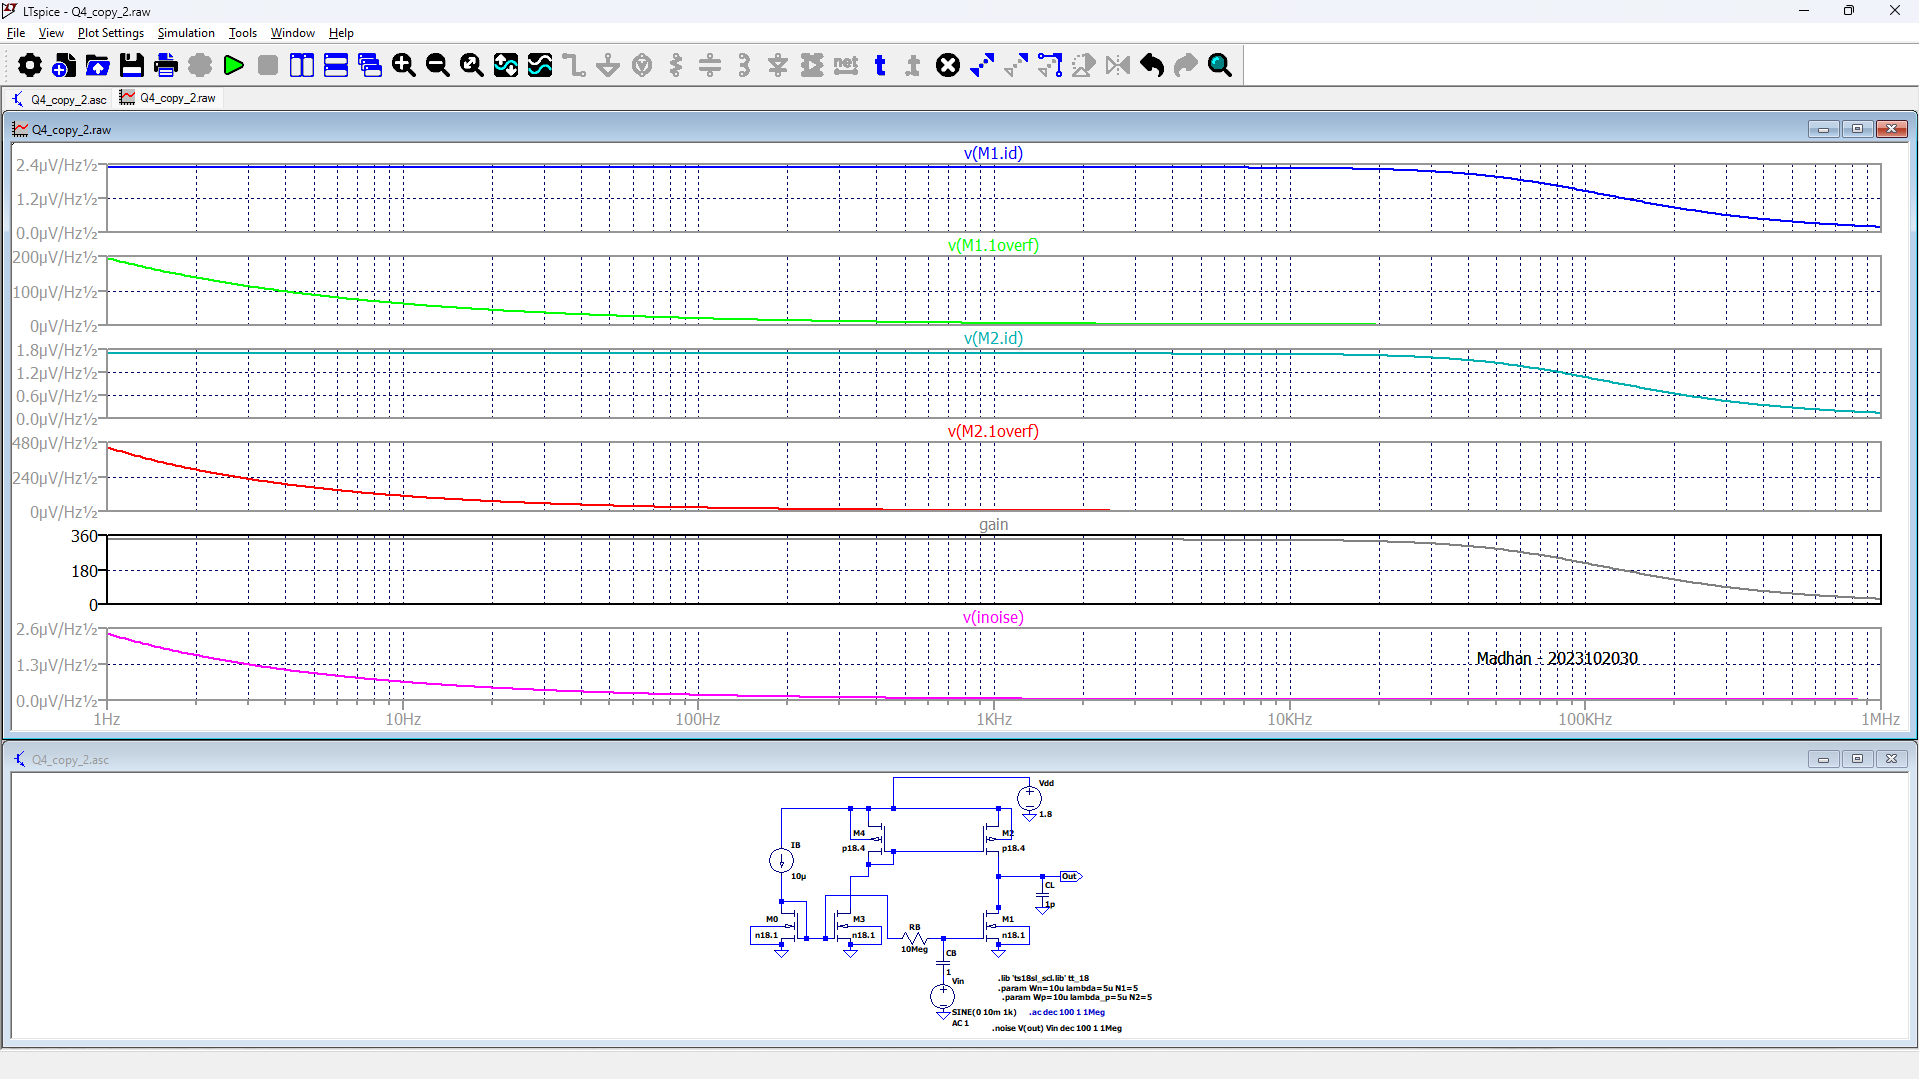
\includegraphics[width=0.9\textwidth]{images/q4_c_3.png}
    \caption{Simulation plots showing Noise PSD, Gain, and Bandwidth for the third case ($W/L = 10\mu/10\mu$).}
\end{figure}

\vspace{0.3cm}
\textbf{Inference from Simulation Data:} \\
By isolating $M_1$ and $M_2$, we evaluate the core amplifier's intrinsic noise performance. First, as the channel length $L$ scales up ($0.18\mu \to 1\mu \to 10\mu$), channel length modulation is reduced, leading to a higher output resistance ($r_o$) and a massively increased mid-band gain ($22.03 \to 336.97$). Second, as the total gate area ($W \times L$) increases, the $1/f$ (flicker) noise contributed by $M_1$ and $M_2$ drops significantly. For instance, $M_1$'s flicker noise drops from $3.95\text{ mV}$ to $681\ \mu\text{V}$. The combination of heavily suppressed flicker noise and much higher voltage gain results in the isolated input-referred RMS noise dropping by over $98\%$, from $239.86 \ \mu\text{V}$ down to just $4.43 \ \mu\text{V}$. 

\textit{Note: The total simulated input-referred noise for the entire circuit was significantly higher in all cases (e.g., $517.65\ \mu\text{V}$ for Case i). This confirms that the biasing network and current mirrors ($M_0, M_3, M_4$) inject a substantial amount of noise into the signal path, validating the theoretical derivation from Part (b).}

\subsection*{(d) NEF Calculation and Tabulation}

The Noise Efficiency Factor (NEF) is calculated using Steyaert's definition:
\begin{equation}
    NEF = v_{n_{in,rms}} \times \sqrt{\frac{2 \times I_{DC}}{\pi \times U_T \times 4kT \times BW}}
\end{equation}
Using the standard room temperature values ($T = 300\text{ K}$), $k = 1.38 \times 10^{-23}\text{ J/K}$, and thermal voltage $U_T = 25.85\text{ mV}$, the NEF for the three simulated designs is tabulated below. The $I_{DC}$ values were extracted directly from the SPICE operating point (.op) simulations to account for non-ideal current mirroring due to channel length modulation.

\begin{figure}[H]
    \centering
    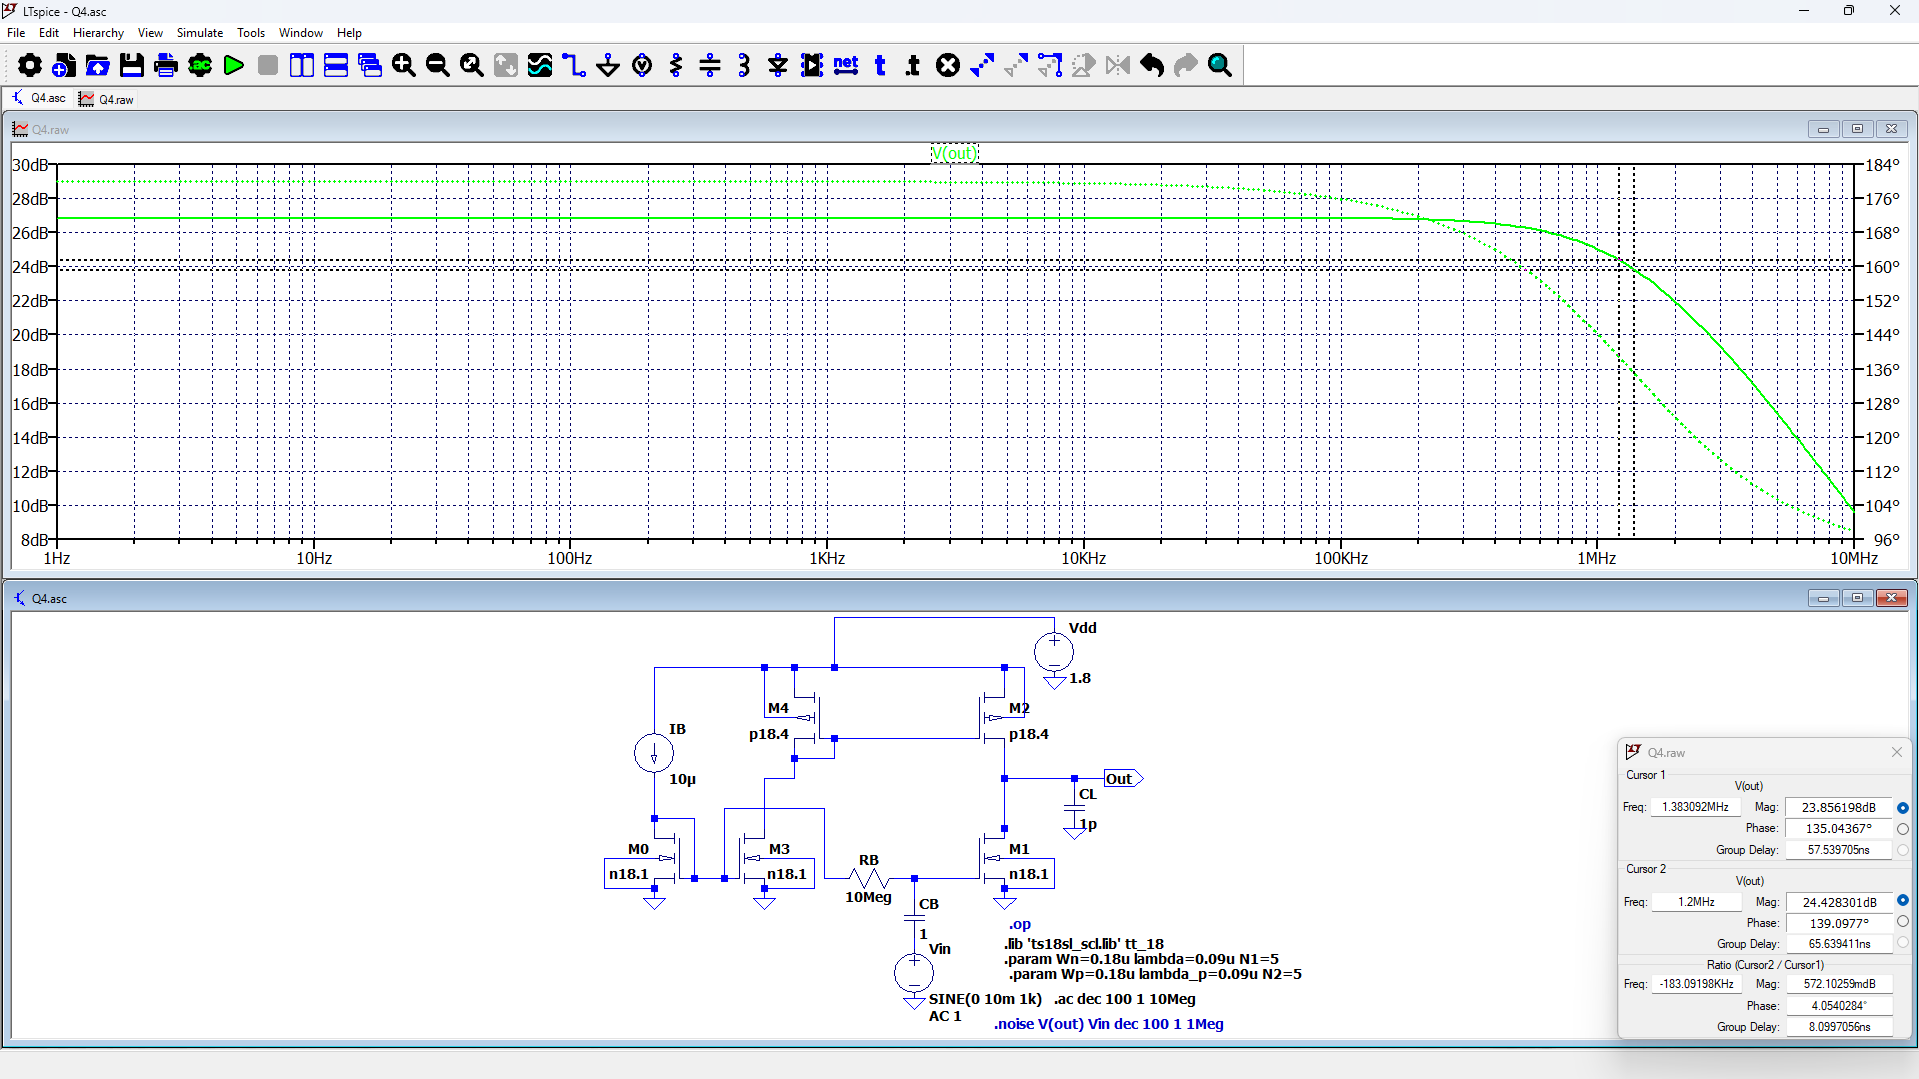
\includegraphics[width=0.9\textwidth]{images/q4_d_1_1.png}
    \caption{Simulation plot showing the AC Gain and -3-dB Bandwidth for the first case ($W/L = 0.18\mu/0.18\mu$).}
\end{figure}

\begin{figure}[H]
    \centering
    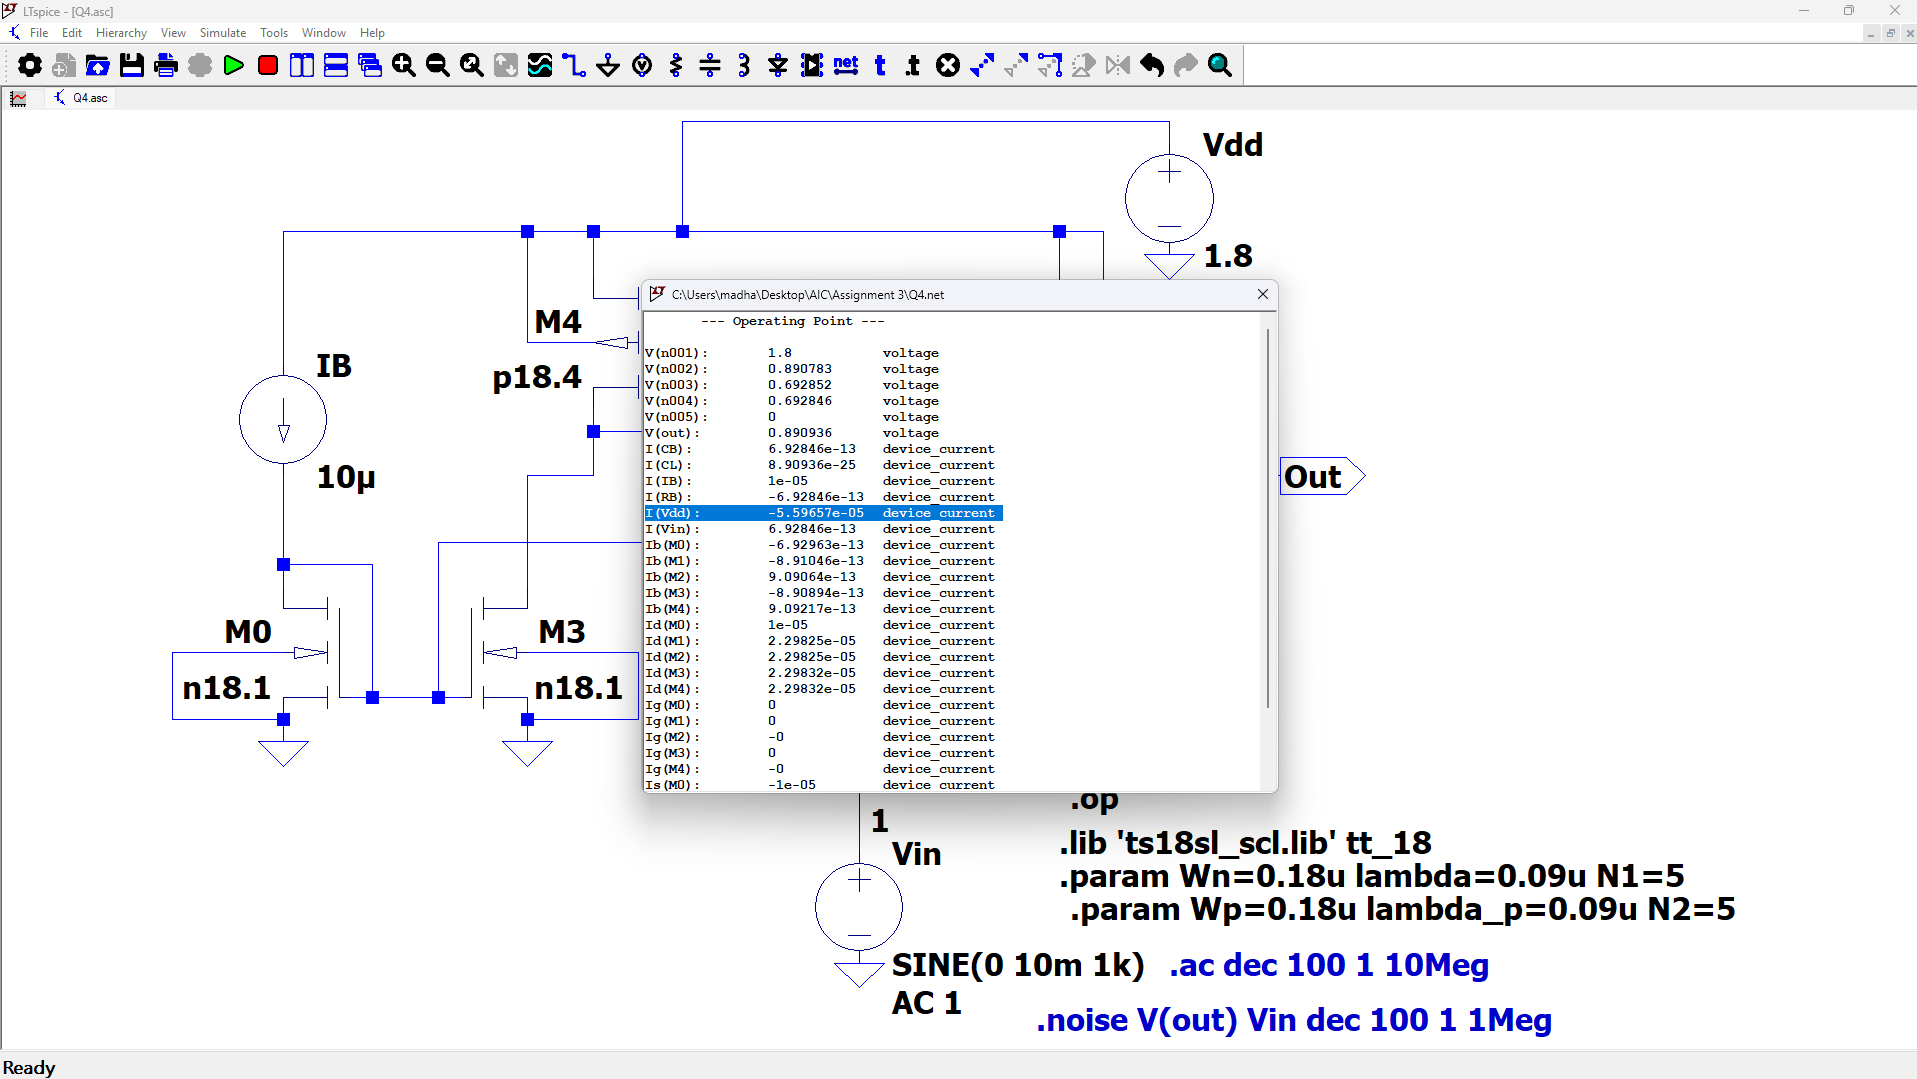
\includegraphics[width=0.9\textwidth]{images/q4_d_1_2.png}
    \caption{Simulation plot showing the DC operating point and extracted $I_{DC}$ for the first case ($W/L = 0.18\mu/0.18\mu$).}
\end{figure}

\begin{figure}[H]
    \centering
    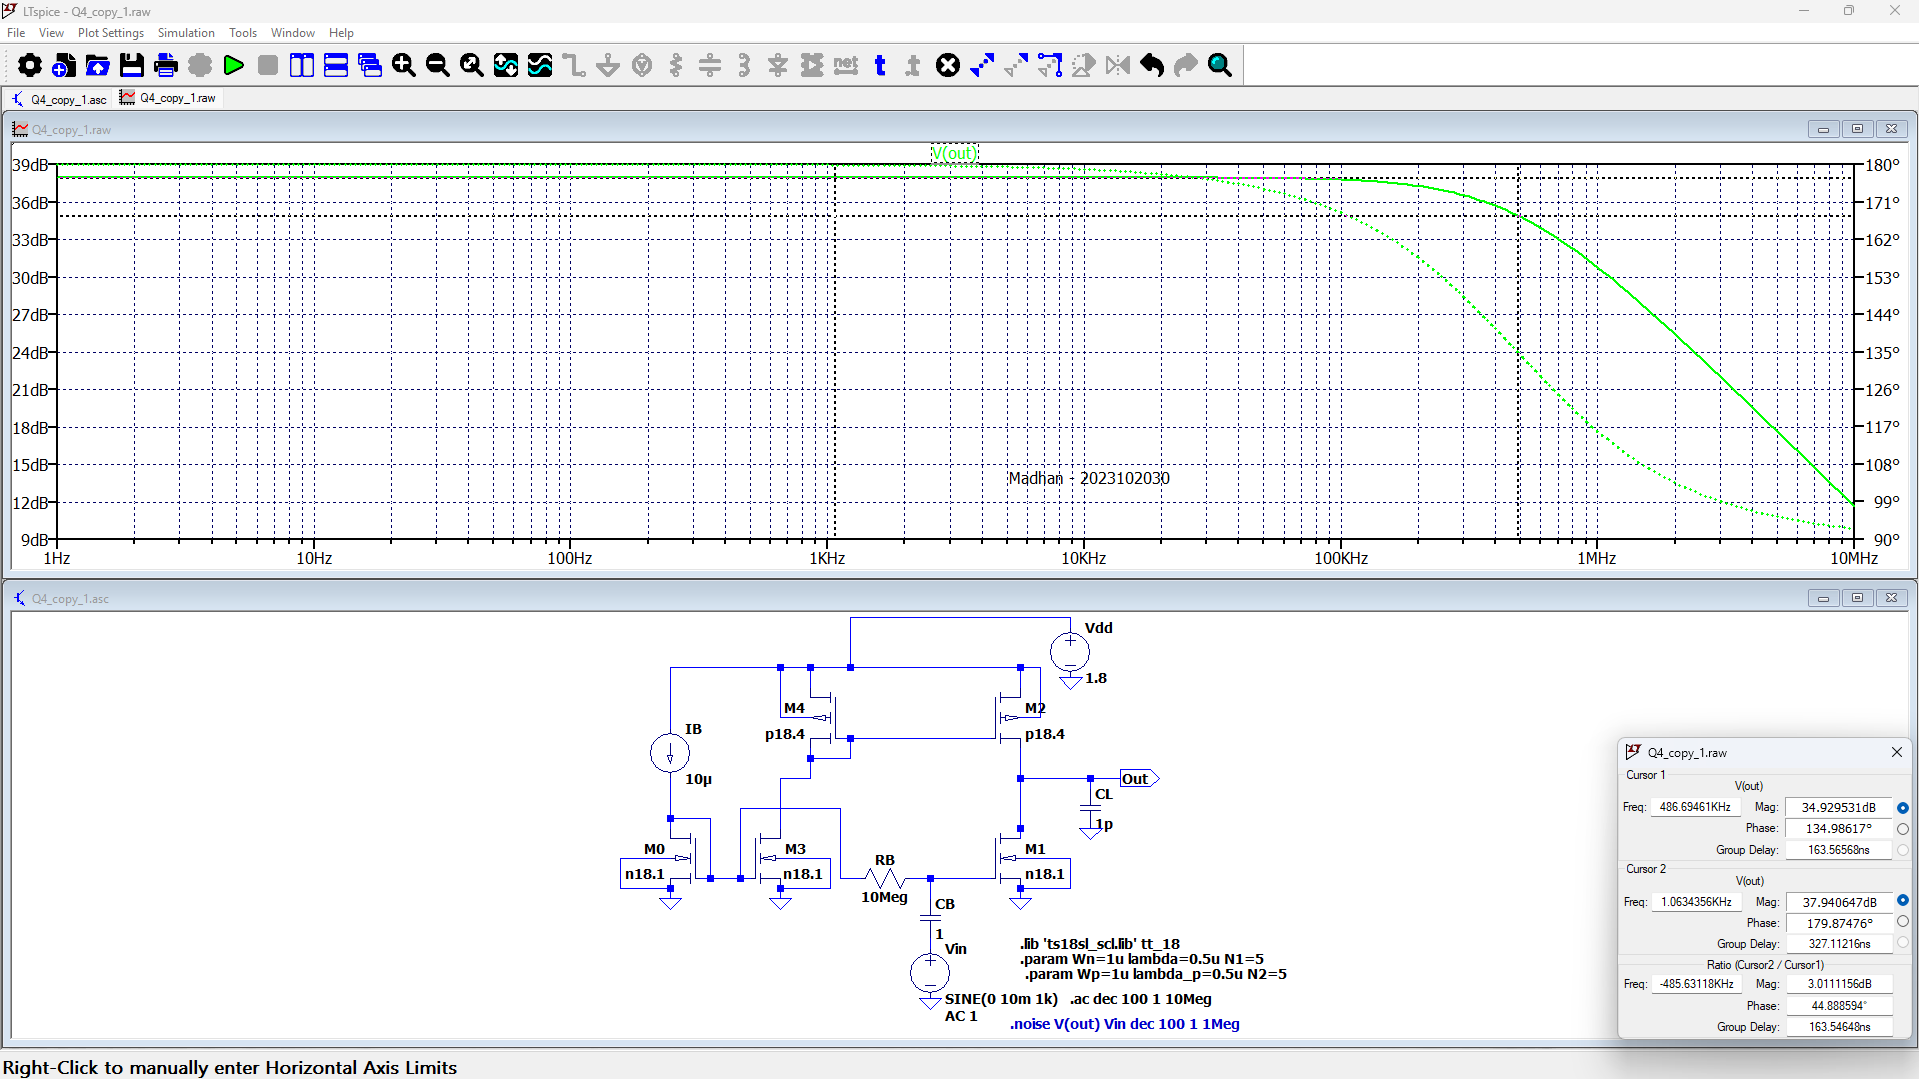
\includegraphics[width=0.9\textwidth]{images/q4_d_2_1.png}
    \caption{Simulation plot showing the AC Gain and -3-dB Bandwidth for the second case ($W/L = 1\mu/1\mu$).}
\end{figure}

\begin{figure}[H]
    \centering
    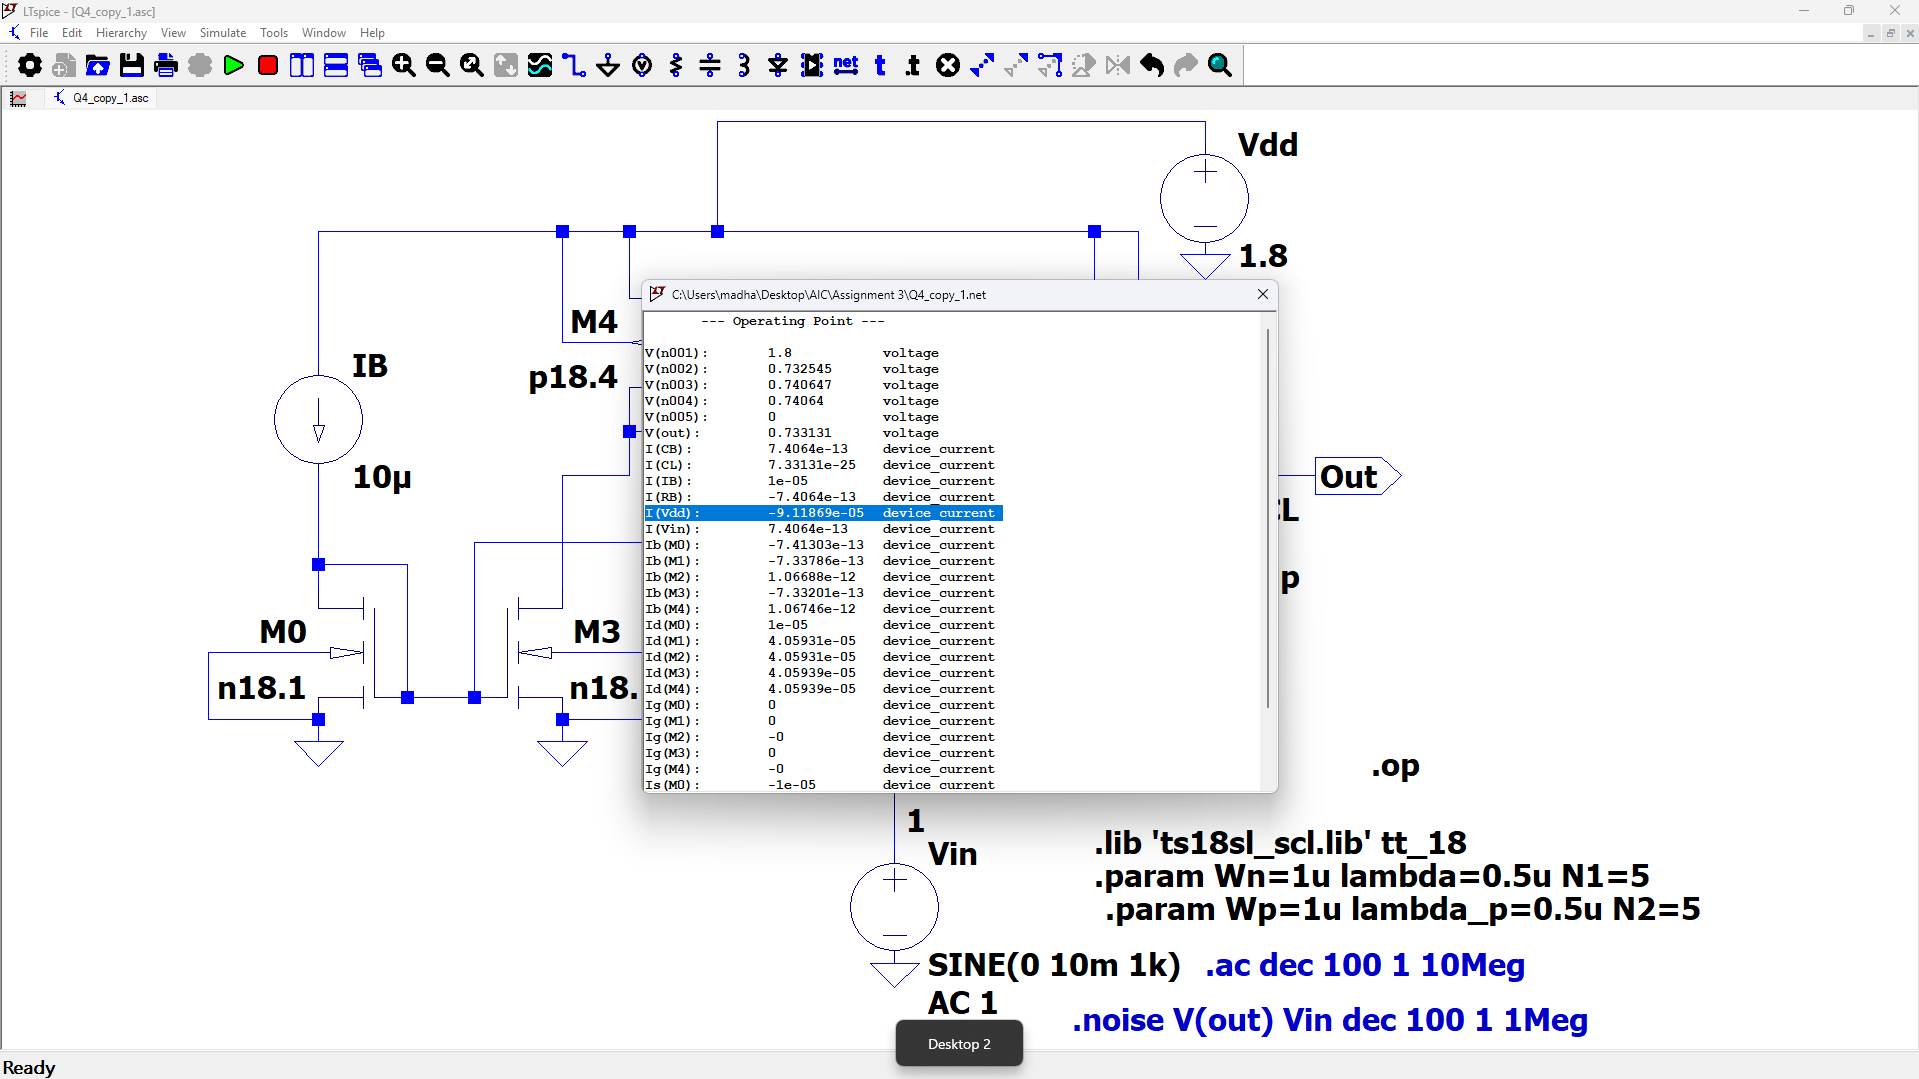
\includegraphics[width=0.9\textwidth]{images/q4_d_2_2.png}
    \caption{Simulation plot showing the DC operating point and extracted $I_{DC}$ for the second case ($W/L = 1\mu/1\mu$).}
\end{figure}

\begin{figure}[H]
    \centering
    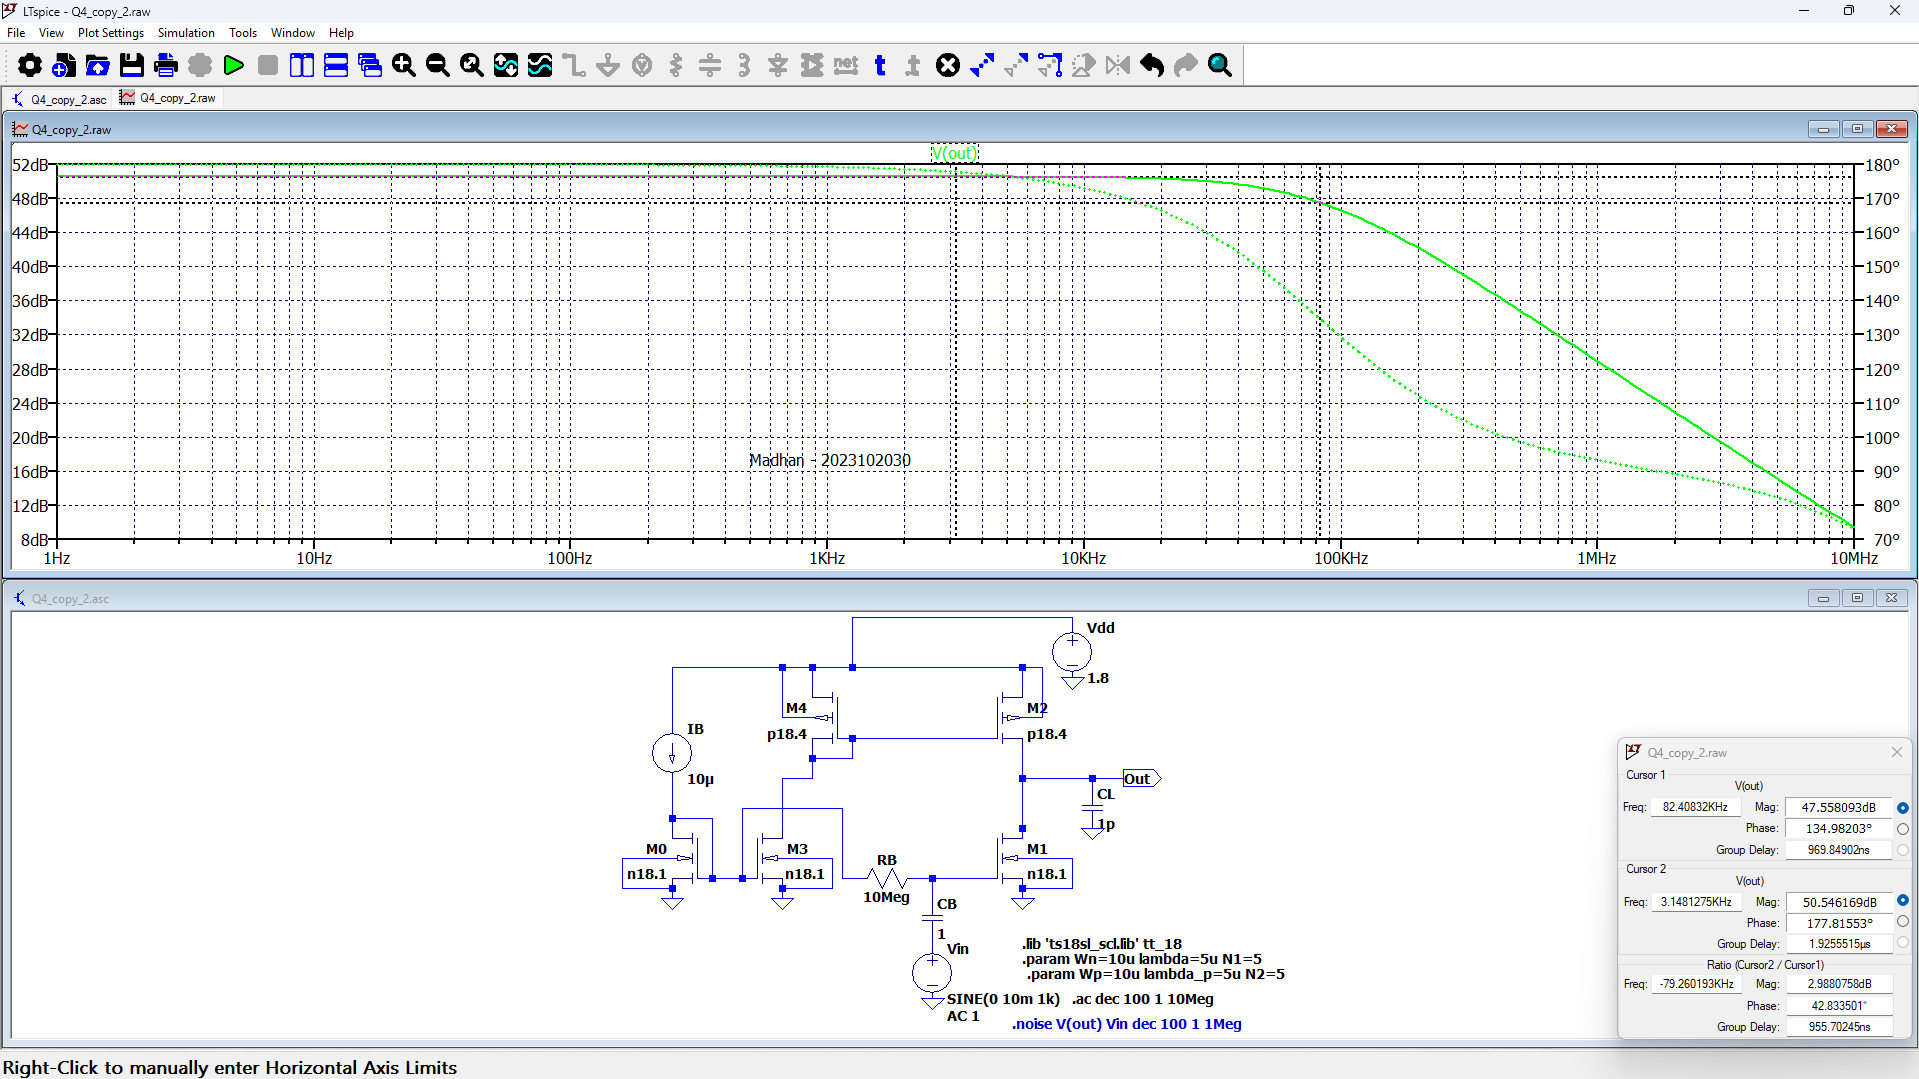
\includegraphics[width=0.9\textwidth]{images/q4_d_3_1.png}
    \caption{Simulation plot showing the AC Gain and -3-dB Bandwidth for the third case ($W/L = 10\mu/10\mu$).}
\end{figure}

\begin{figure}[H]
    \centering
    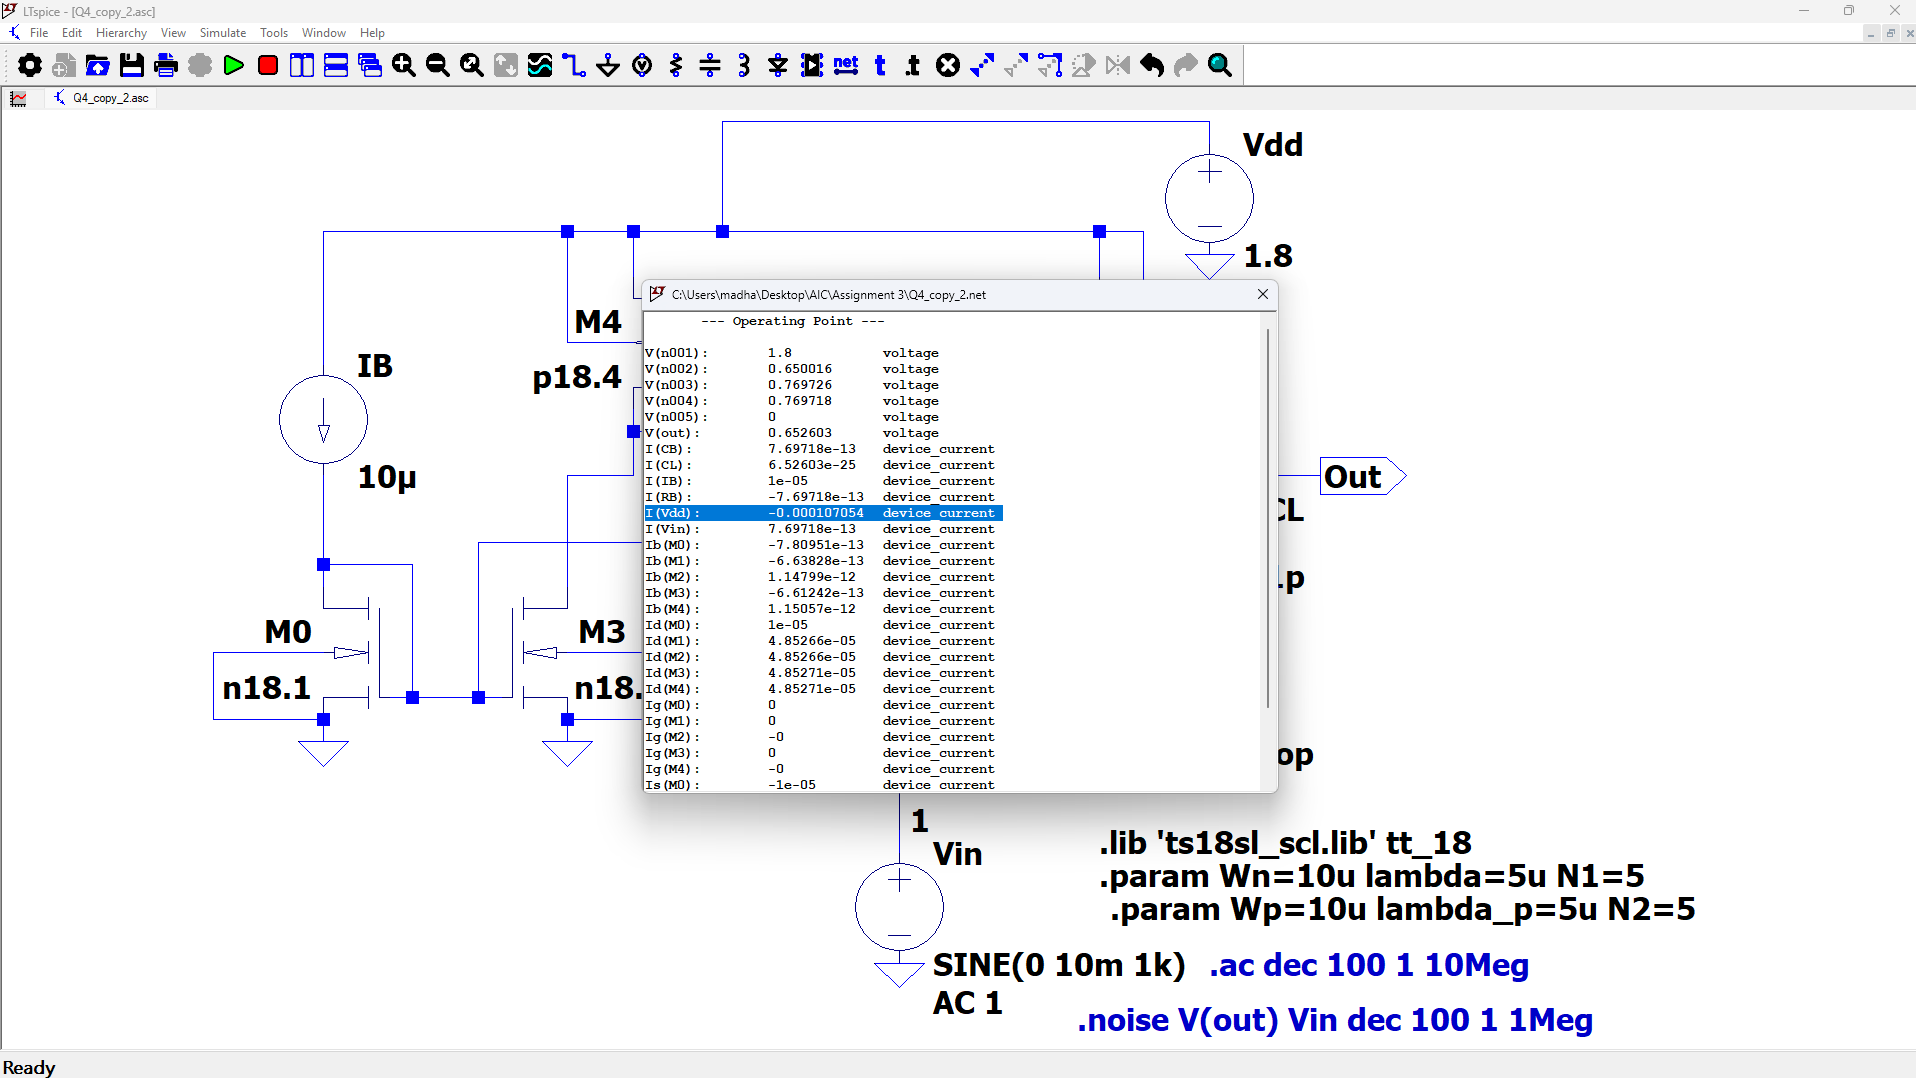
\includegraphics[width=0.9\textwidth]{images/q4_d_3_2.png}
    \caption{Simulation plot showing the DC operating point and extracted $I_{DC}$ for the third case ($W/L = 10\mu/10\mu$).}
\end{figure}

\begin{table}[H]
    \centering
    \caption{Noise Efficiency Factor for the Three Designs}
    \renewcommand{\arraystretch}{1.4}
    \resizebox{\textwidth}{!}{
    \begin{tabular}{@{}ccccccc@{}}
        \toprule
        \textbf{Design} & \textbf{Gain (V/V)} & \textbf{Amp BW (-3-dB)} & \textbf{$I_{DC}$} & \textbf{$v_{n_{in,rms}}$ (Due to $M_1, M_2$)} & \textbf{NEF} \\
        \midrule
        1 (Case i)   & $22.03$  & $1.383 \text{ MHz}$  & $55.97 \ \mu\text{A}$ & $239.86 \ \mu\text{V}$ & $\mathbf{58.80}$ \\
        2 (Case ii)  & $78.89$  & $486.69 \text{ kHz}$ & $91.19 \ \mu\text{A}$ & $34.06 \ \mu\text{V}$  & $\mathbf{17.98}$ \\
        3 (Case iii) & $336.97$ & $82.41 \text{ kHz}$  & $107.05 \ \mu\text{A}$ & $4.43 \ \mu\text{V}$  & $\mathbf{6.16}$ \\
        \bottomrule
    \end{tabular}}
\end{table}

\textbf{Inference:} 
The NEF dramatically improves (decreases) as the transistor area scales up. While the larger devices ($10\mu$) suffer a significant reduction in bandwidth due to parasitic capacitance, the massive reduction in $1/f$ noise and the vast increase in open-loop gain entirely dominate the Steyaert equation, driving the NEF down to a highly efficient 6.16.


\subsection*{(e) Proposed Modification to Reduce NEF}

\textbf{Proposed Modification:} Convert the circuit into an \textbf{Inverter-Based (Current-Reused) Amplifier}. 

\textbf{Explanation of Trade-off Improvement:} 
In the standard differential/common-source topology explored in previous sections, the PMOS load ($M_2$) acts strictly as an active current source. It consumes a significant portion of the total static current ($I_{DC}$) and contributes heavily to the total output noise (as shown in Part 4c), but provides \textit{zero} signal transconductance. 

By AC-coupling the input signal $v_{in}$ to the gate of $M_2$ alongside $M_1$, $M_2$ acts as an active amplifying device rather than a passive load. The effective transconductance of the stage doubles ($G_{m,tot} = g_{m1} + g_{m2}$). This drastically increases the voltage gain for the exact same DC current budget. Because the input-referred noise is inversely proportional to $G_{m,tot}^2$, this modification heavily suppresses the noise floor without requiring additional power, yielding a much lower NEF.

\textbf{Assumption:} The $M_2$ PMOS device is sized to compensate the mobility difference, ensuring $g_{m2} \approx g_{m1}$ at the same bias current. This allows us to achieve a near doubling of transconductance without increasing $I_{DC}$.\\
From simulations $\mu_{N} \approx 4\mu_{P}$, so we can size $M_2$ to be 4 times wider than $M_1$ to achieve $g_{m2} \approx g_{m1}$.

\begin{figure}[H]
    \centering
    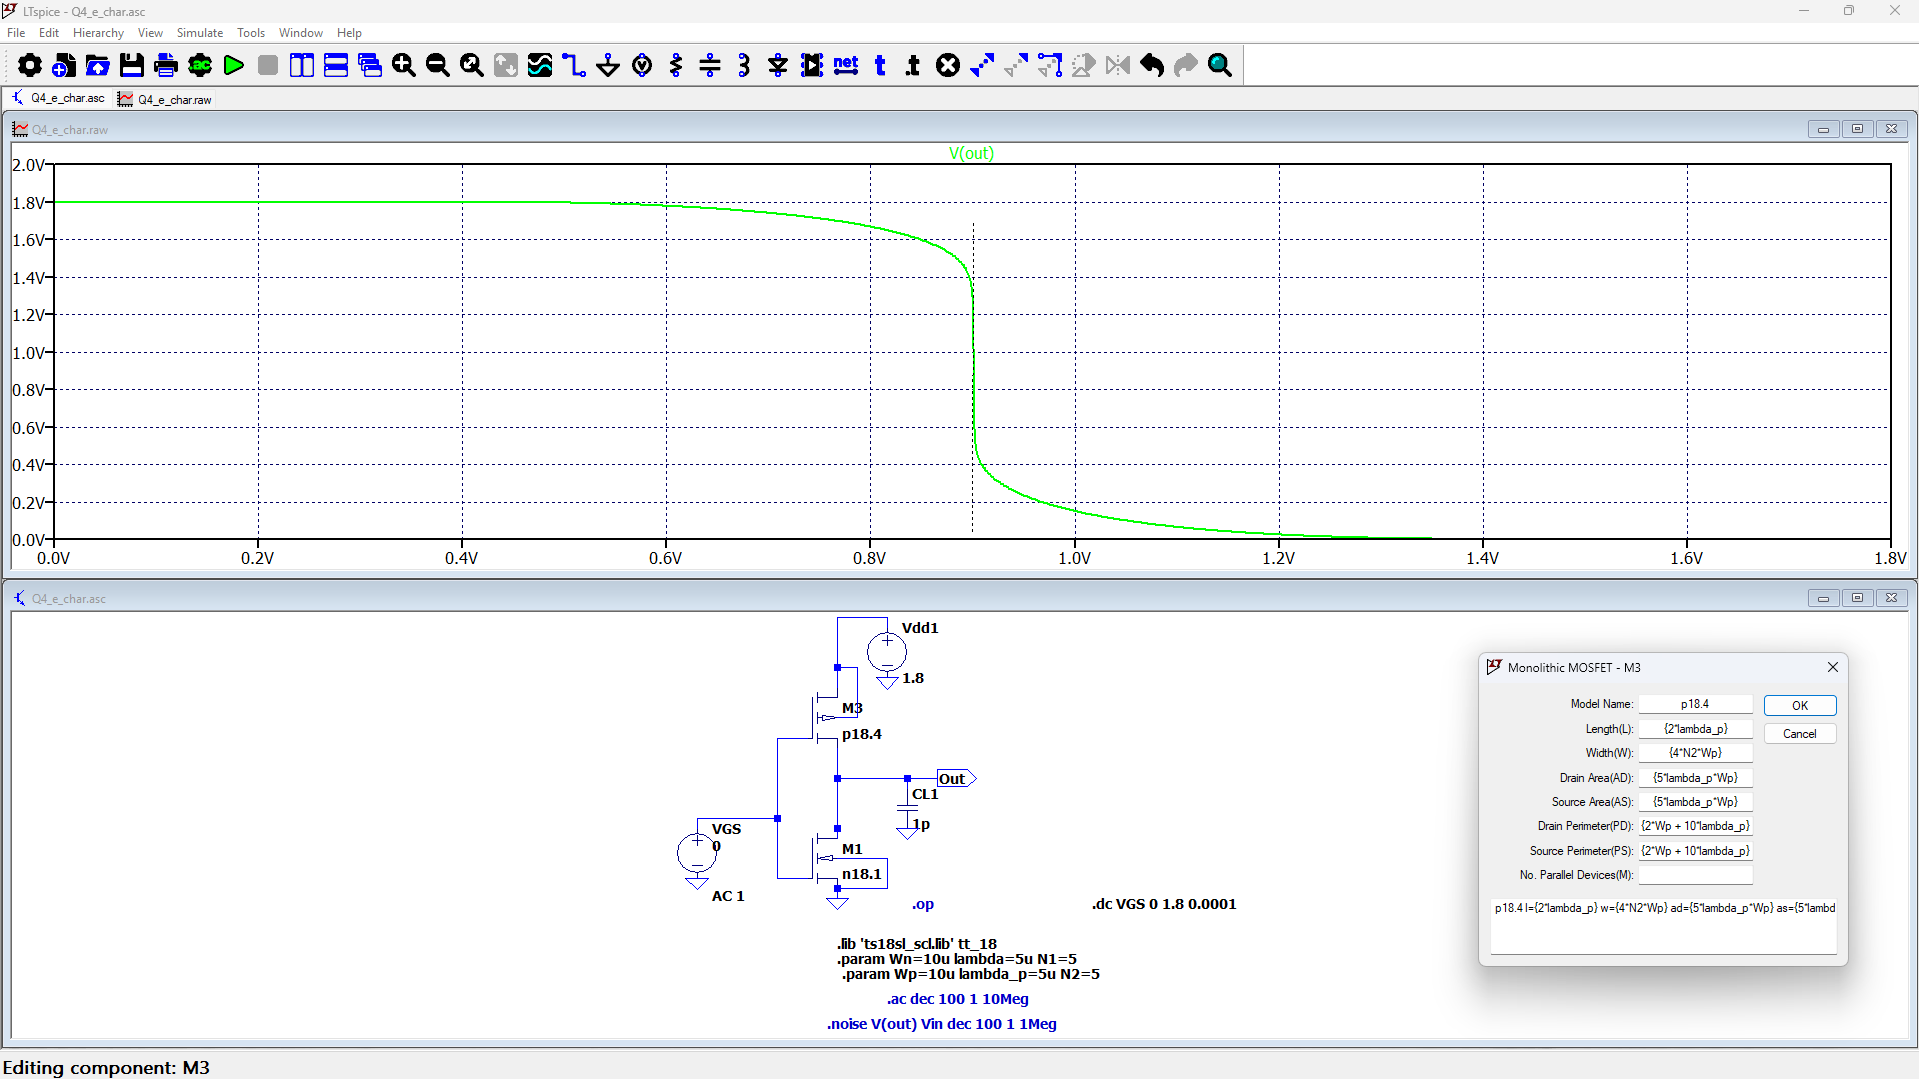
\includegraphics[width=0.8\textwidth]{images/q4_e_char.png}
    \caption{Schematic of the proposed Inverter characterization for the modified amplifier design.}
\end{figure}

\begin{figure}[H]
    \centering
    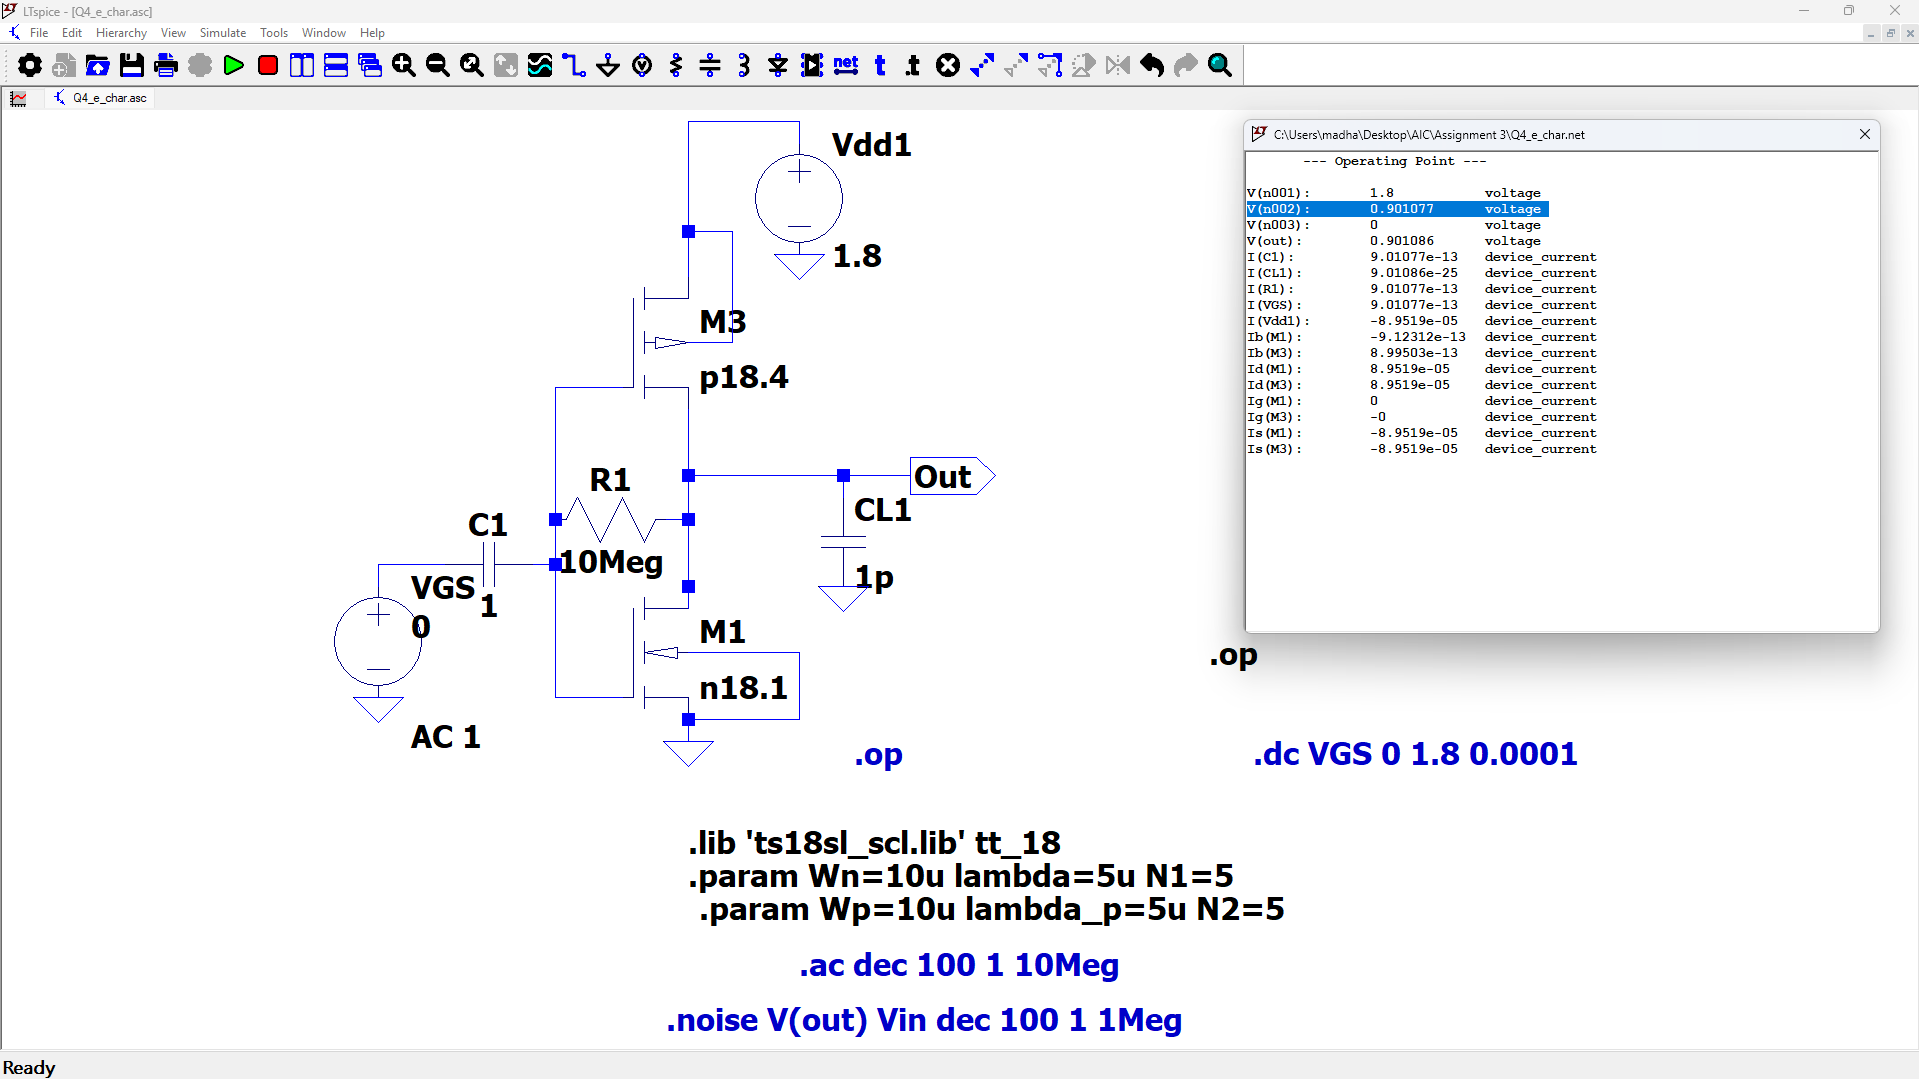
\includegraphics[width=0.8\textwidth]{images/q4_e_bias.png}
    \caption{DC operating point simulation showing the bias currents and voltages for the modified design}
\end{figure}

Similar plots are generated for all three cases: $W/L = 0.18\mu/0.18\mu$, $1\mu/1\mu$, and $10\mu/10\mu$. Which gave the $V_{GS}$ values as follows : 0.91247 V, 0.902054 V, 0.901077 V respecteively. $I_{B}$ value is adjusted acccordingly for different sizings to maintain the respective bias voltage at the gate of $M_1$ and $M_2$ to ensure the maximum steep slope of the I-V curve for both devices, which is the optimal bias point for noise performance (gives the maximum gain which is the dominant factor in reducing the input-referred noise). 

\vspace{0.3cm}
\textbf{Simulation Results \& Detailed Calculations:} \\
The modified circuit was simulated under identical device sizing cases (with $W_P = 4 W_N$). The total RMS output noise was extracted by squaring and summing the uncorrelated thermal and flicker noise components from $M_1$ and $M_2$. This was then divided by the new linear mid-band gain to calculate the improved $v_{n_{in,rms}}$. 

For the NEF calculations, the theoretical denominator constant evaluated at $T=300\text{ K}$ is:
\begin{equation}
    \pi \times U_T \times 4kT = \pi \times 0.02585 \times 4(1.38\times 10^{-23})(300) \approx 1.345 \times 10^{-21}
\end{equation}

\textbf{Case 1: $W/L = 0.18\mu / 0.18\mu$}
\begin{itemize}
    \item \textbf{Linear Gain:} $A_v = 10^{(28.268/20)} = 25.91\text{ V/V}$
    \item \textbf{Output Noise:} $v_{n,out} = \sqrt{(2916.2)^2 + (90.9)^2 + (2108.6)^2 + (110.4)^2} \approx 3601.5\ \mu\text{V}$
    \item \textbf{Input-Referred Noise:} $v_{n_{in,rms}} = 3601.5 / 25.91 = \mathbf{139.0\ \mu\text{V}}$
    \item \textbf{NEF:} $139.0\times 10^{-6} \times \sqrt{\frac{2 \times 109.3\times 10^{-6}}{1.345\times 10^{-21} \times 4.198\times 10^6}} = \mathbf{27.35}$
\end{itemize}

\textbf{Case 2: $W/L = 1\mu / 1\mu$}
\begin{itemize}
    \item \textbf{Linear Gain:} $A_v = 10^{(40.447/20)} = 105.03\text{ V/V}$
    \item \textbf{Output Noise:} $v_{n,out} = \sqrt{(1424.2)^2 + (292.0)^2 + (1122.1)^2 + (317.9)^2} \approx 1863.8\ \mu\text{V}$
    \item \textbf{Input-Referred Noise:} $v_{n_{in,rms}} = 1863.8 / 105.03 = \mathbf{17.75\ \mu\text{V}}$
    \item \textbf{NEF:} $17.75\times 10^{-6} \times \sqrt{\frac{2 \times 112.06\times 10^{-6}}{1.345\times 10^{-21} \times 1.062\times 10^6}} = \mathbf{7.03}$
\end{itemize}

\textbf{Case 3: $W/L = 10\mu / 10\mu$}
\begin{itemize}
    \item \textbf{Linear Gain:} $A_v = 10^{(56.020/20)} = 632.39\text{ V/V}$
    \item \textbf{Output Noise:} $v_{n,out} = \sqrt{(764.9)^2 + (765.1)^2 + (638.1)^2 + (821.7)^2} \approx 1500.9\ \mu\text{V}$
    \item \textbf{Input-Referred Noise:} $v_{n_{in,rms}} = 1500.9 / 632.39 = \mathbf{2.37\ \mu\text{V}}$
    \item \textbf{NEF:} $2.37\times 10^{-6} \times \sqrt{\frac{2 \times 107.91\times 10^{-6}}{1.345\times 10^{-21} \times 114.8\times 10^3}} = \mathbf{2.80}$
\end{itemize}

\begin{figure}[H]
    \centering
    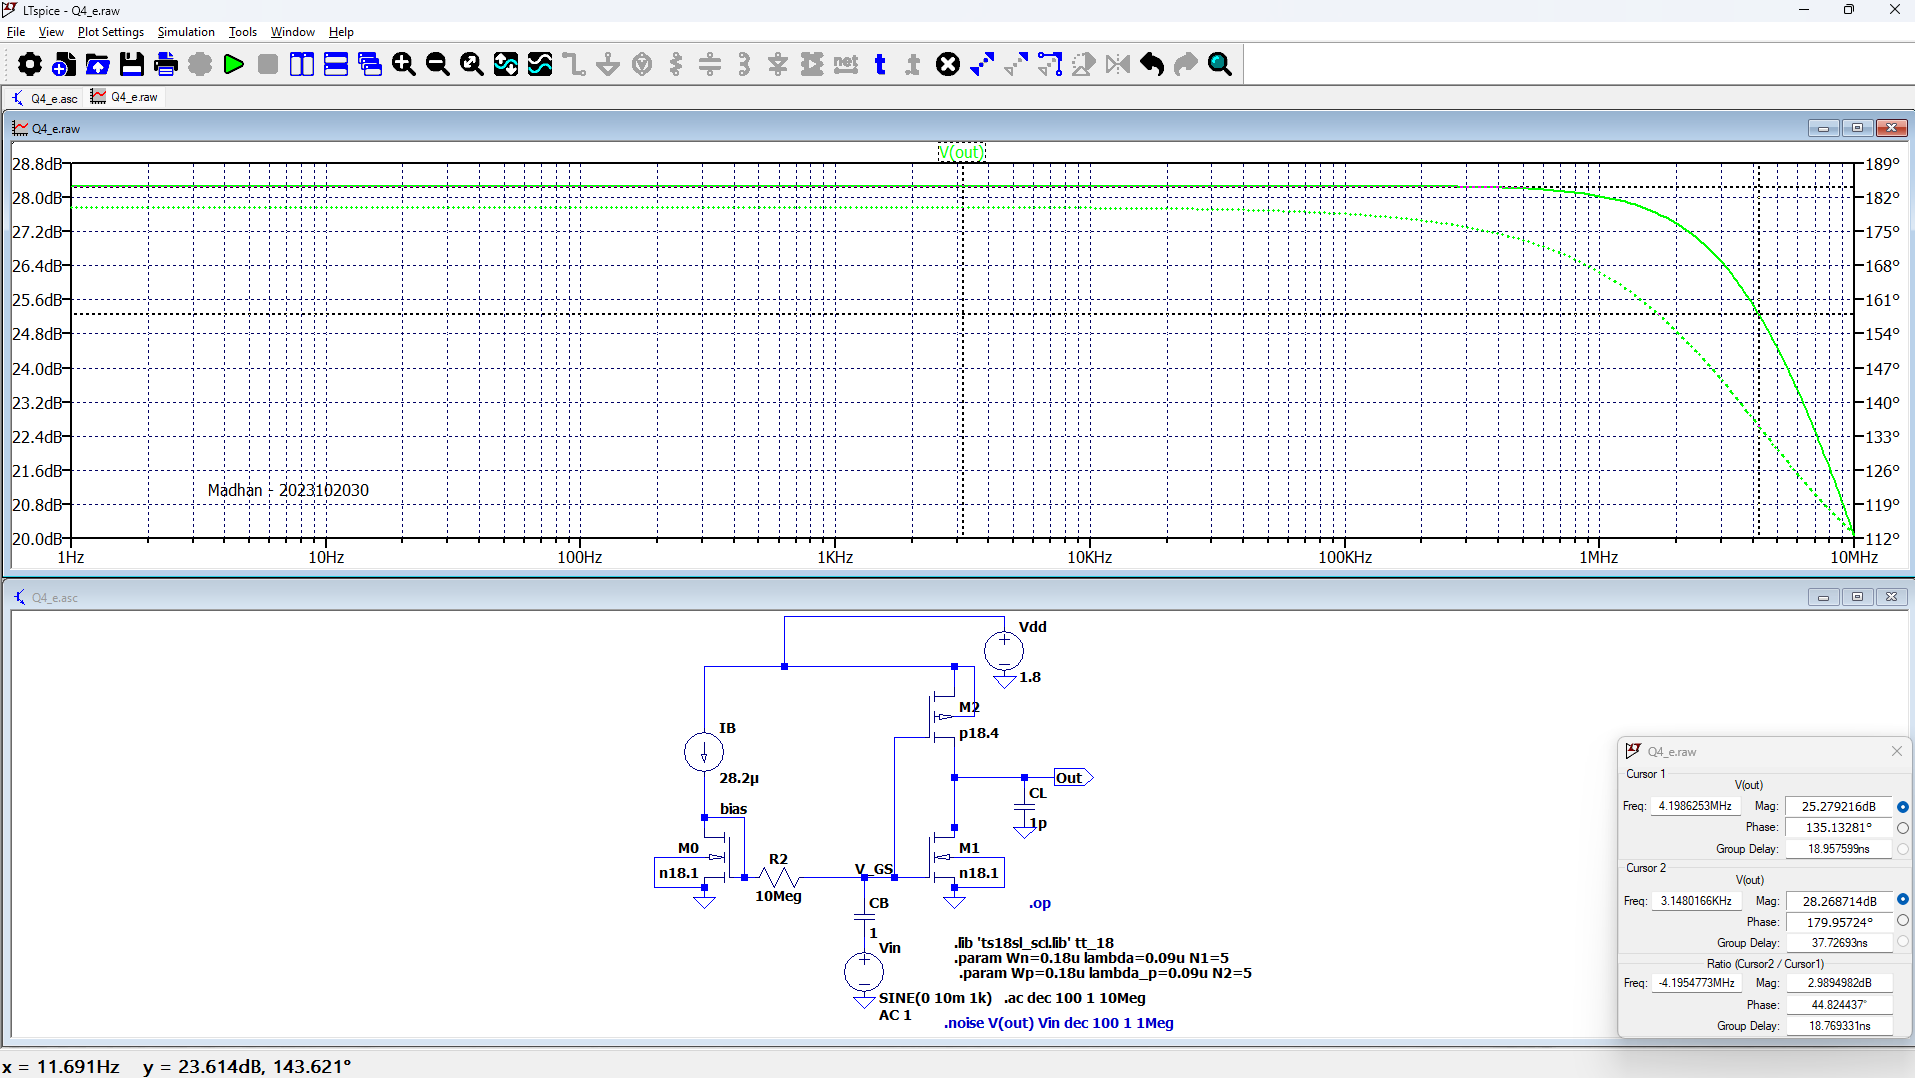
\includegraphics[width=0.8\textwidth]{images/q4_e_1_1.png}
    \caption{AC Gain and -3-dB Bandwidth for the modified design with $W/L = 0.18\mu/0.18\mu$.}
\end{figure}

\begin{figure}[H]
    \centering
    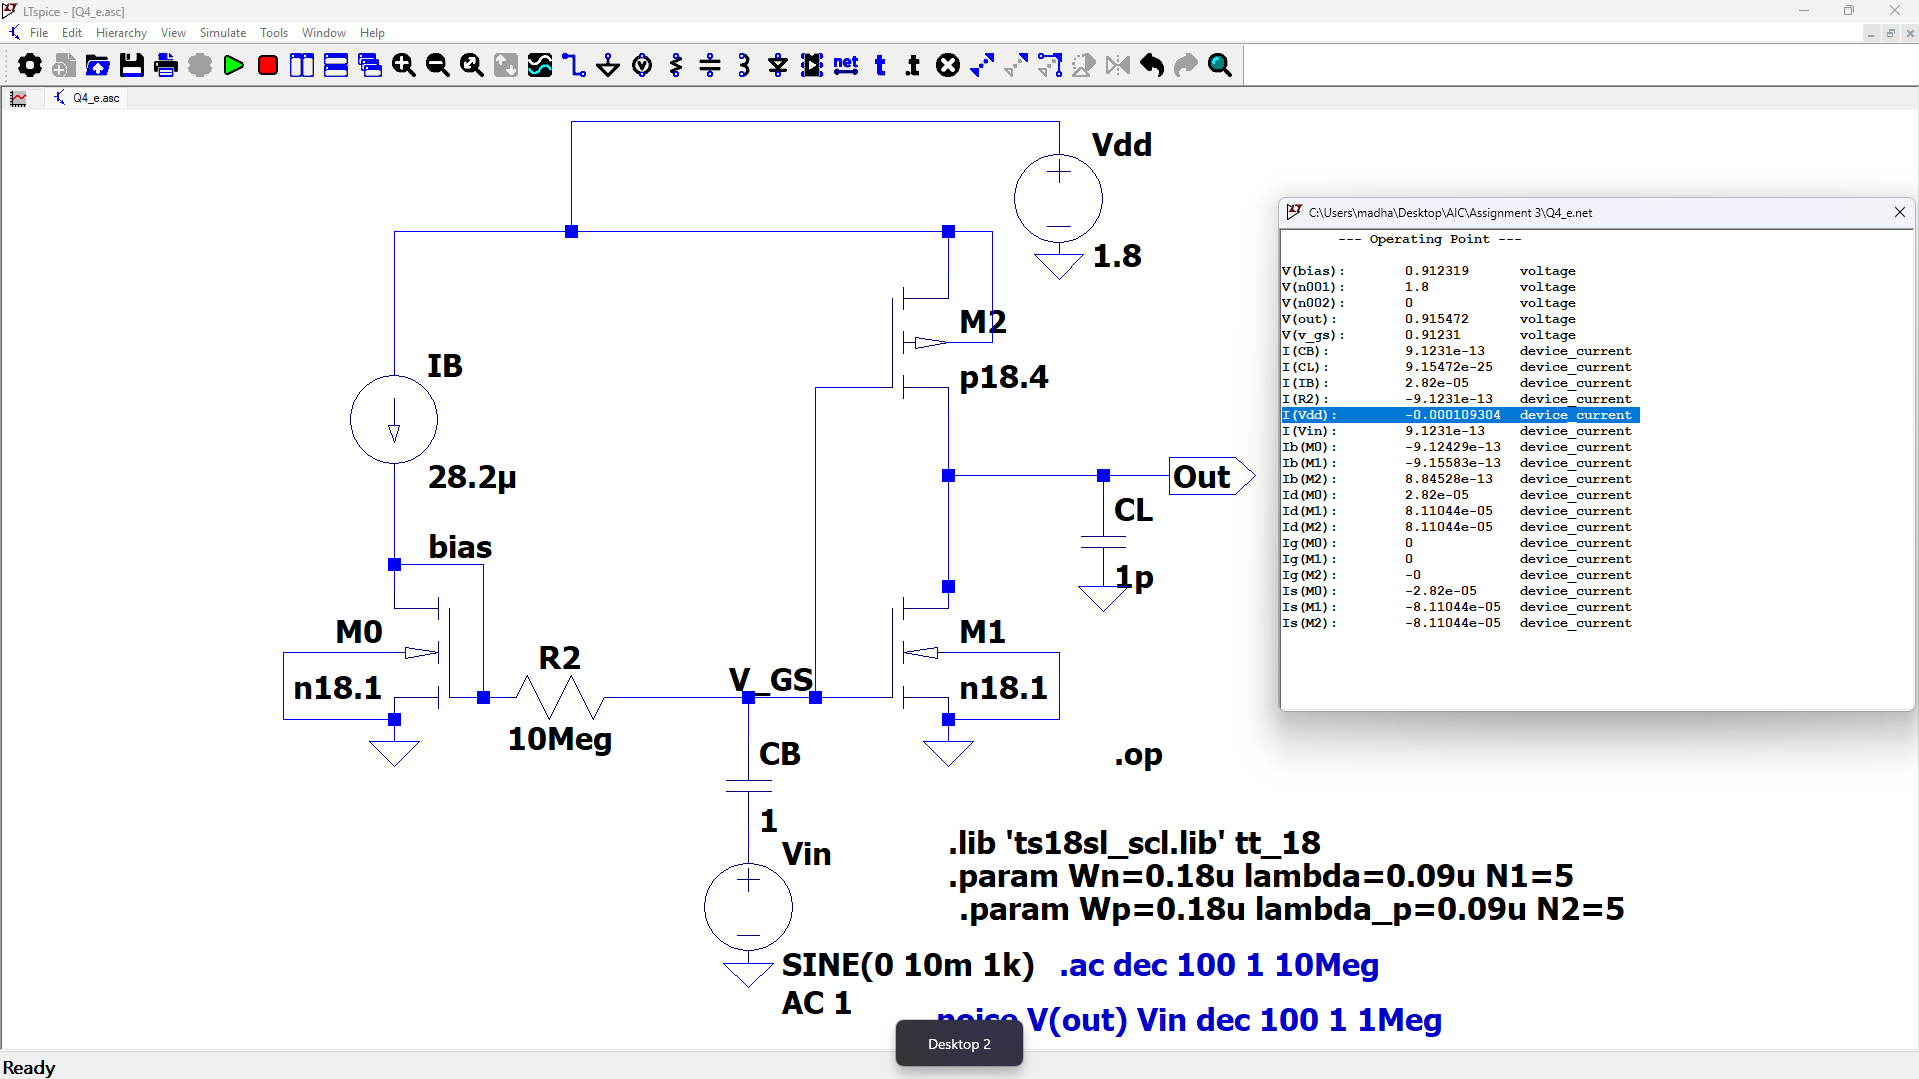
\includegraphics[width=0.8\textwidth]{images/q4_e_1_2.png}
    \caption{Operating point and extracted $I_{DC}$ for the modified design with $W/L = 0.18\mu/0.18\mu$.}
\end{figure}

\begin{figure}[H]
    \centering
    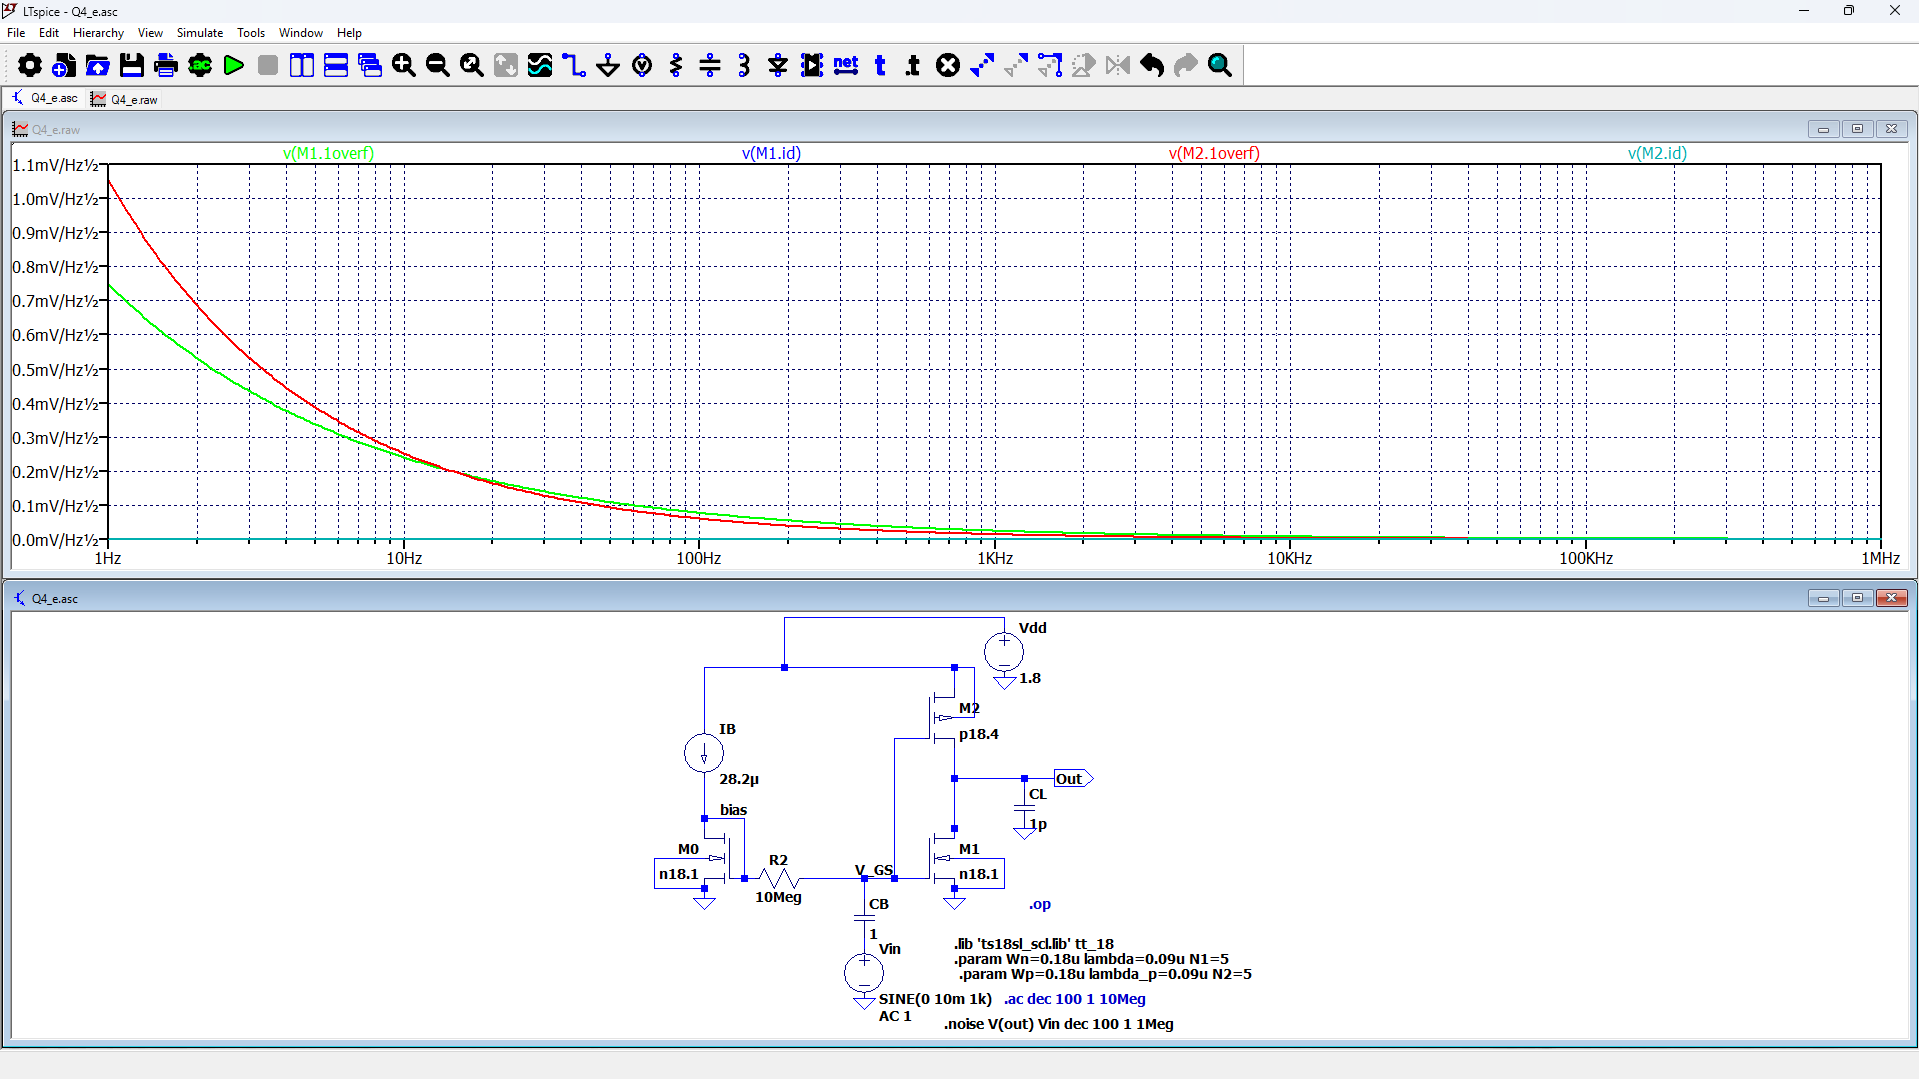
\includegraphics[width=0.8\textwidth]{images/q4_e_1_3.png}
    \caption{Noise PSD of M1 and M2 for the modified design with $W/L = 0.18\mu/0.18\mu$.}
\end{figure}

\begin{figure}[H]
    \centering
    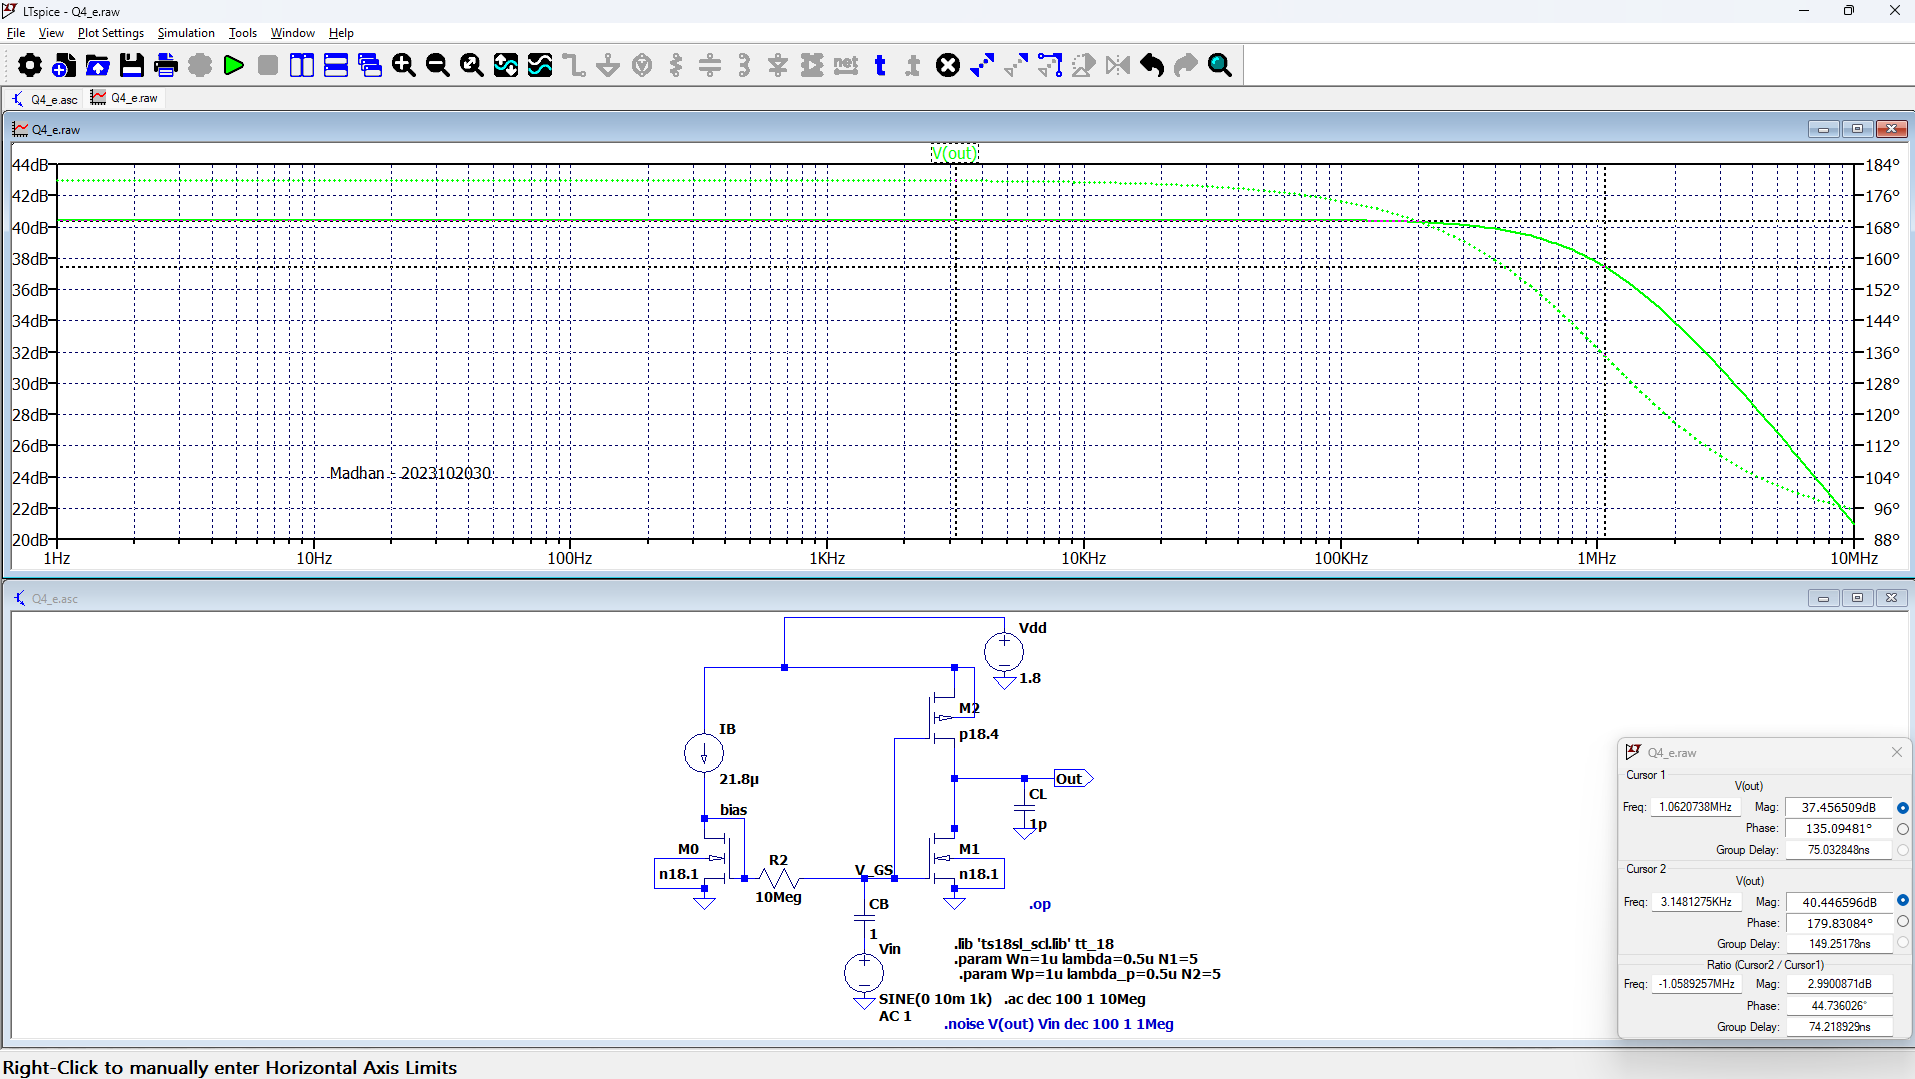
\includegraphics[width=0.8\textwidth]{images/q4_e_2_1.png}
    \caption{AC Gain and -3-dB Bandwidth for the modified design with $W/L = 1\mu/1\mu$.}
\end{figure}

\begin{figure}[H]
    \centering
    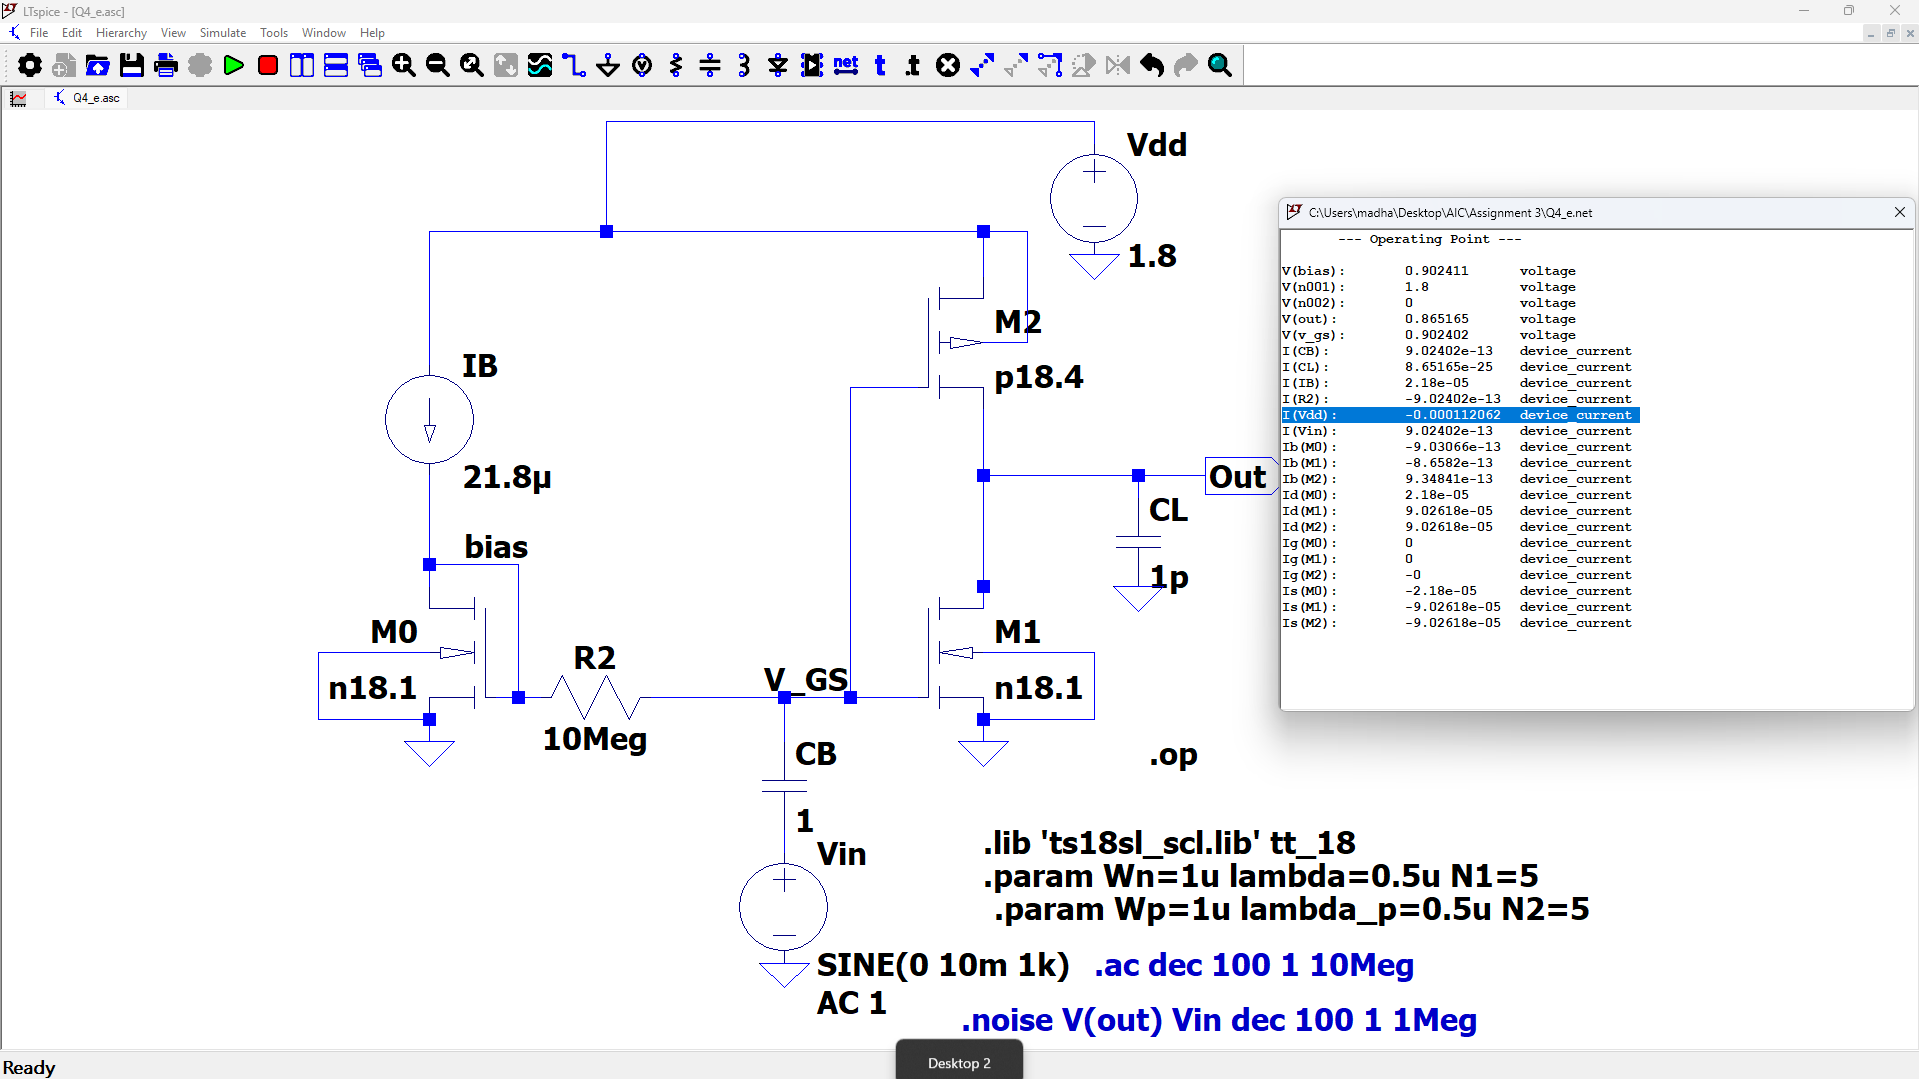
\includegraphics[width=0.8\textwidth]{images/q4_e_2_2.png}
    \caption{Operating point and extracted $I_{DC}$ for the modified design with $W/L = 1\mu/1\mu$.}
\end{figure}

\begin{figure}[H]
    \centering
    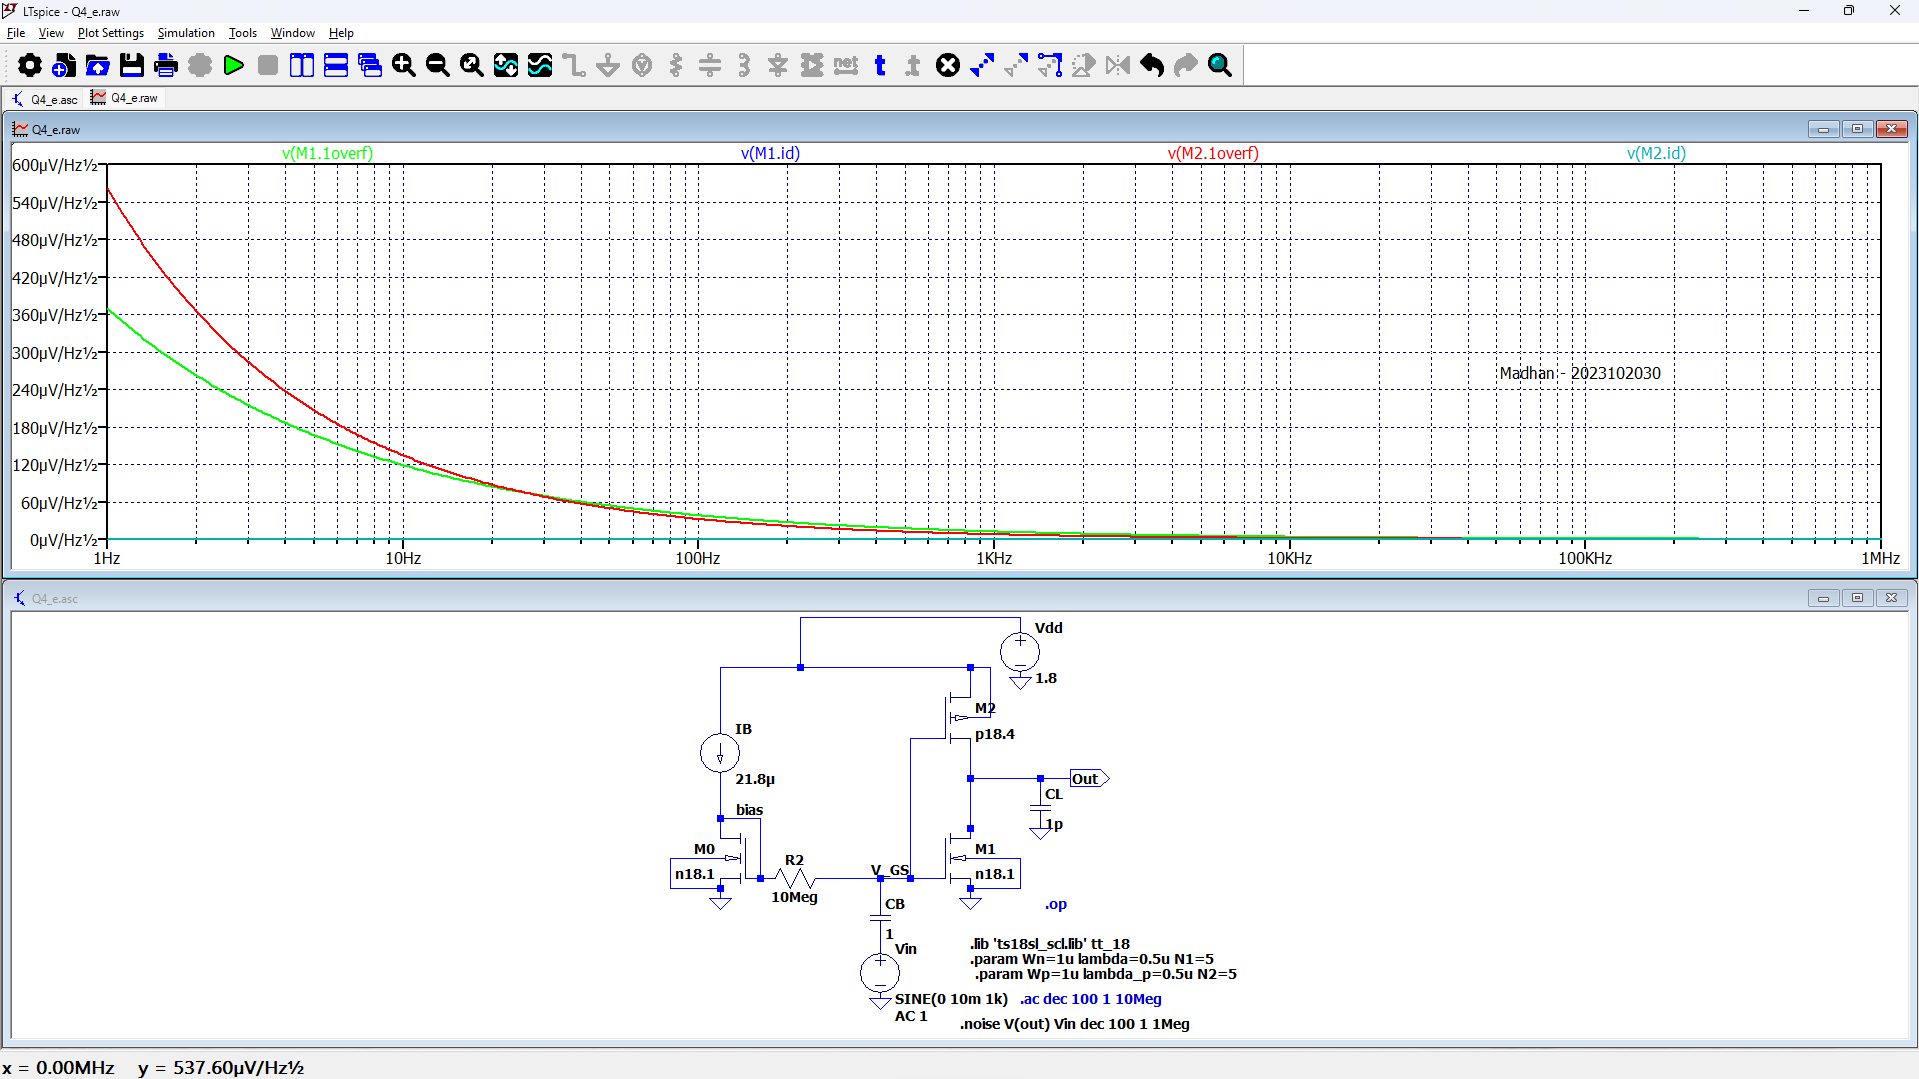
\includegraphics[width=0.8\textwidth]{images/q4_e_2_3.png}
    \caption{Noise PSD of M1 and M2 for the modified design with $W/L = 1\mu/1\mu$.}
\end{figure}

\begin{figure}[H]
    \centering
    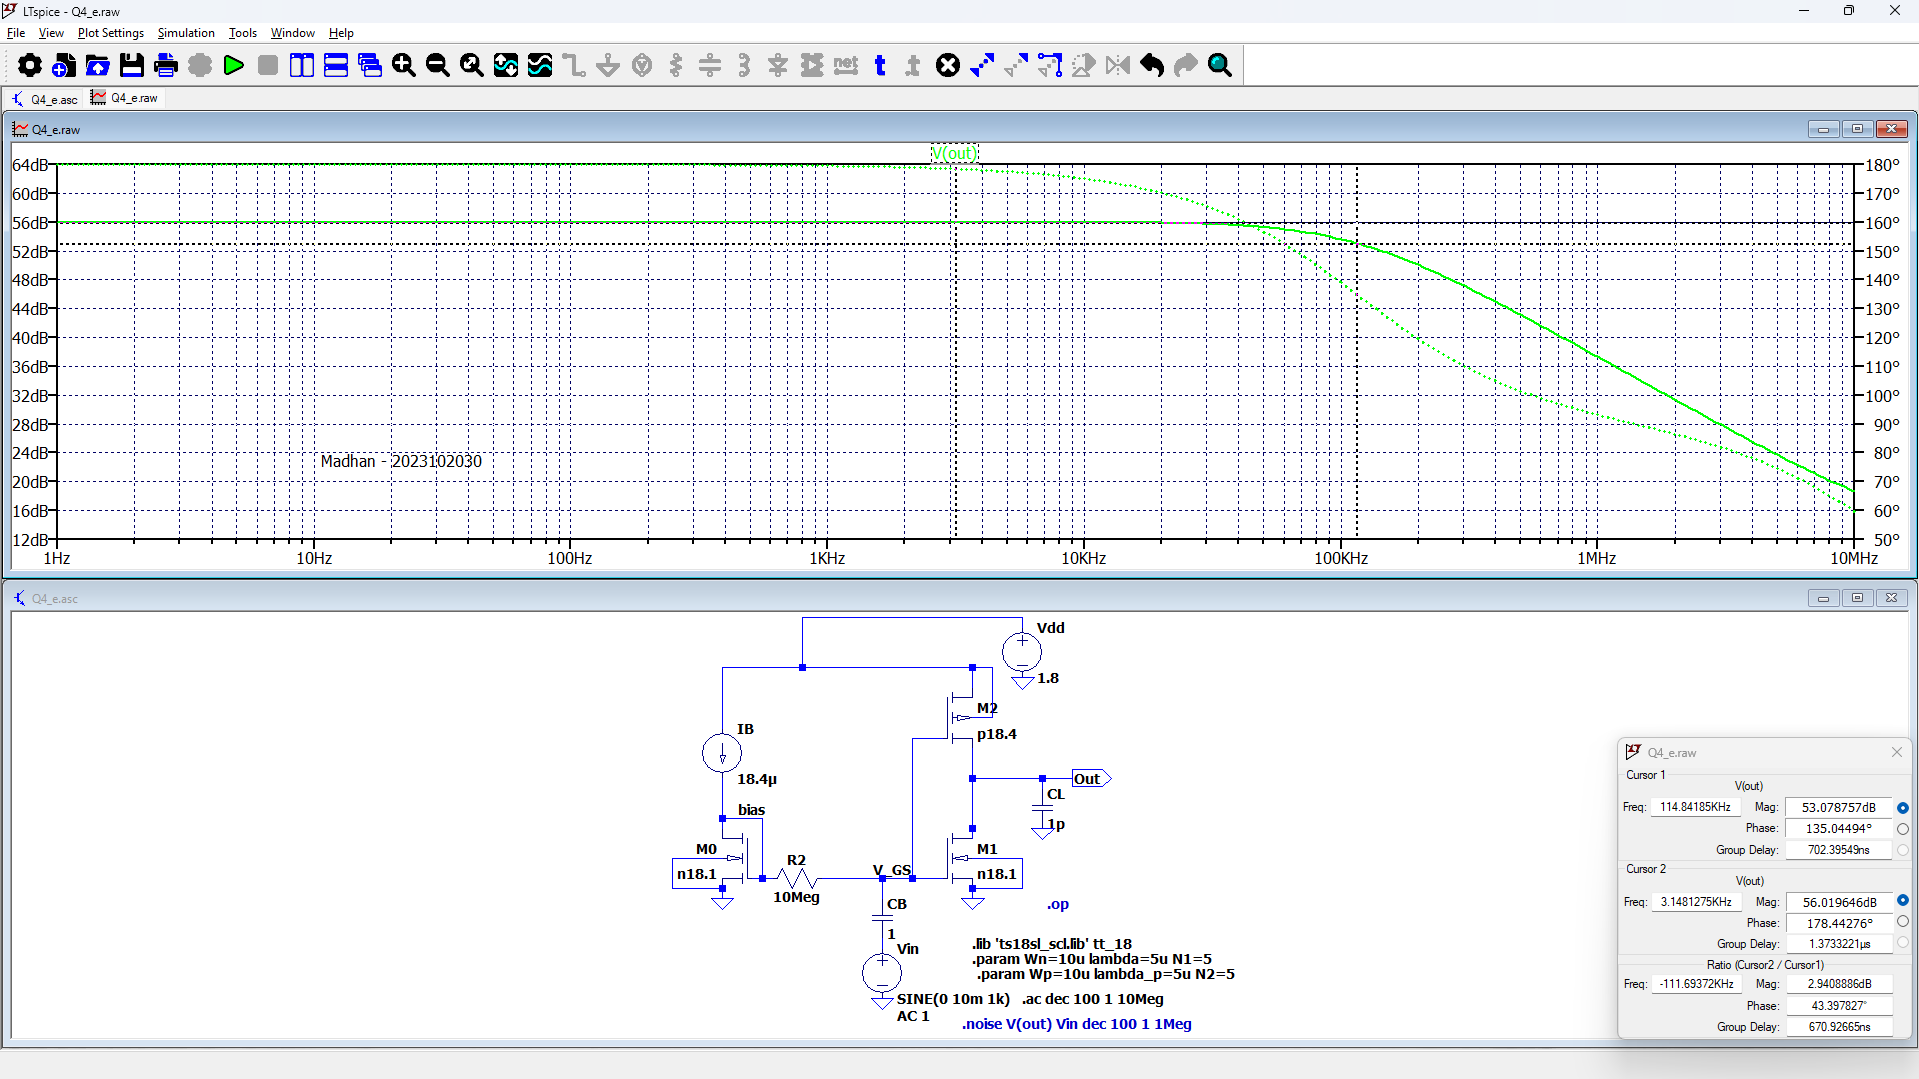
\includegraphics[width=0.8\textwidth]{images/q4_e_3_1.png}
    \caption{AC Gain and -3-dB Bandwidth for the modified design with $W/L = 10\mu/10\mu$.}
\end{figure}

\begin{figure}[H]
    \centering
    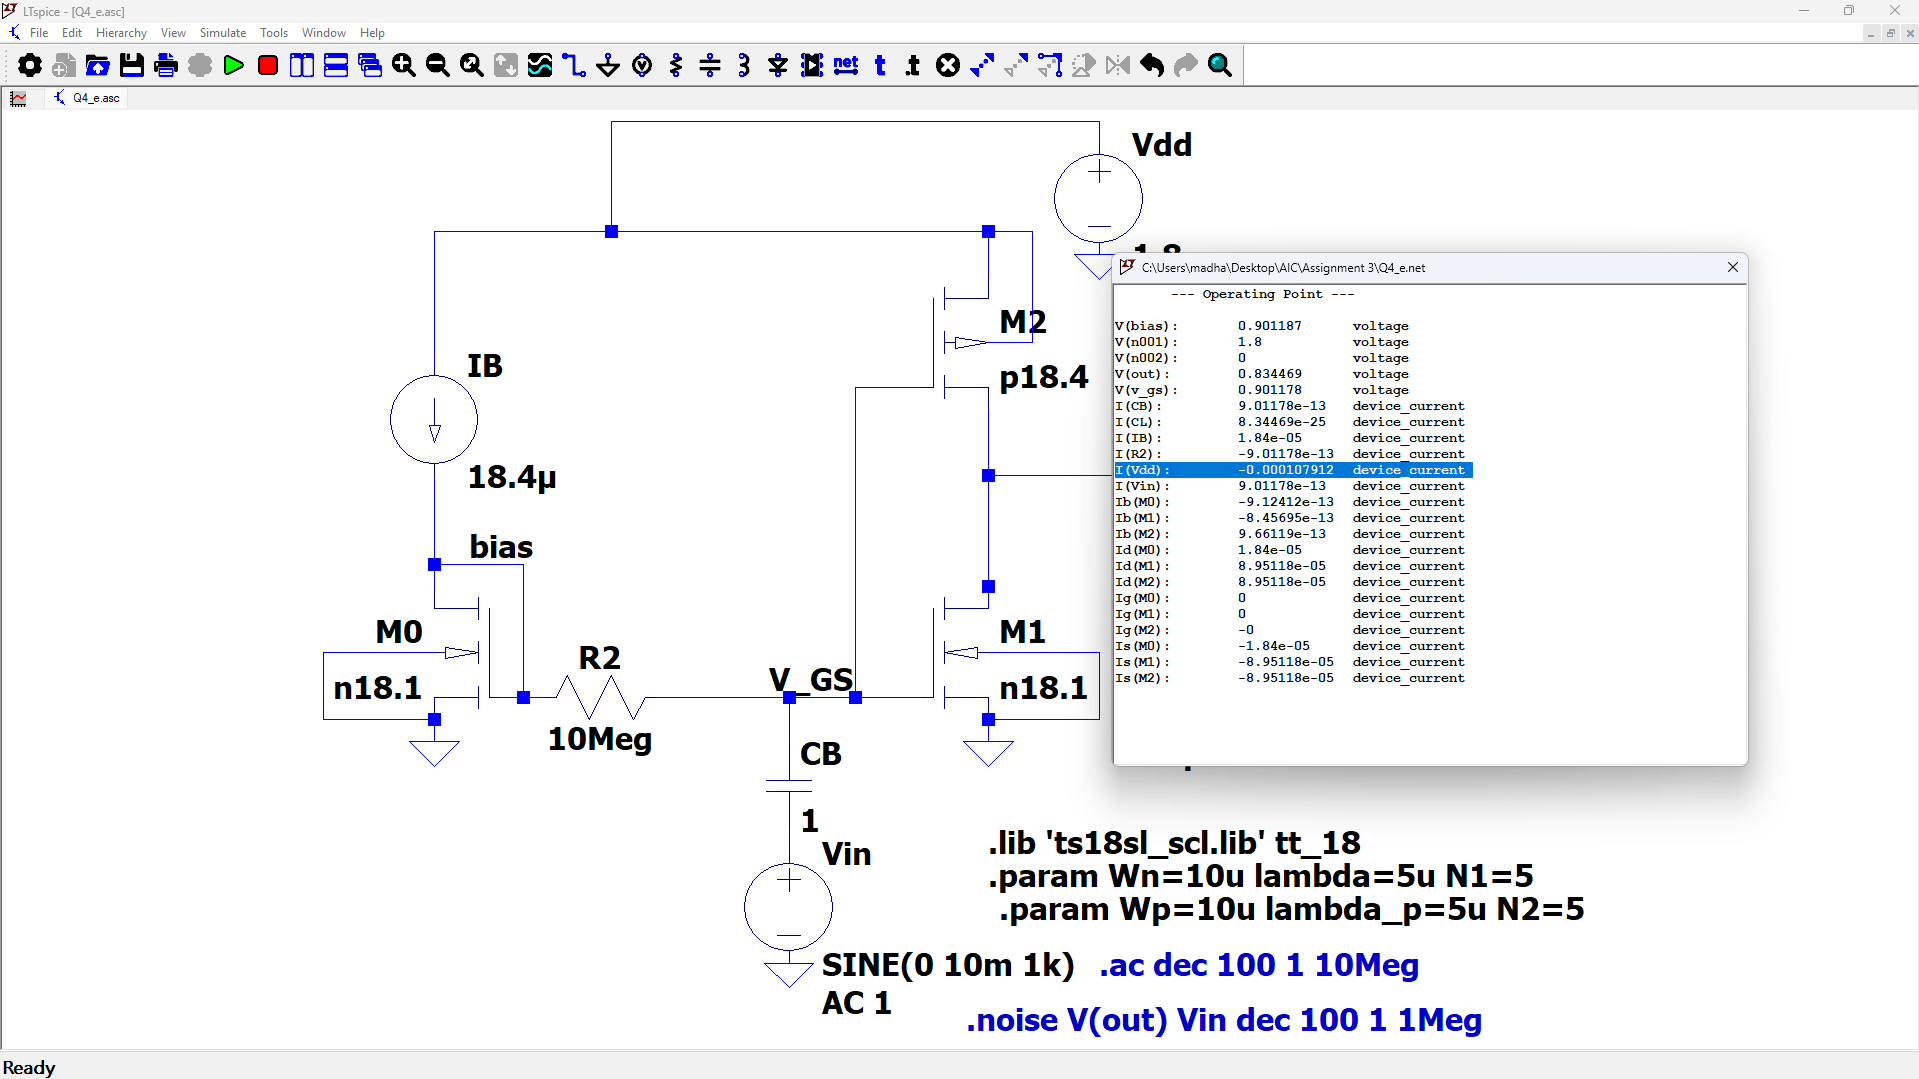
\includegraphics[width=0.8\textwidth]{images/q4_e_3_2.png}
    \caption{Operating point and extracted $I_{DC}$ for the modified design with $W/L = 10\mu/10\mu$.}
\end{figure}

\begin{figure}[H]
    \centering
    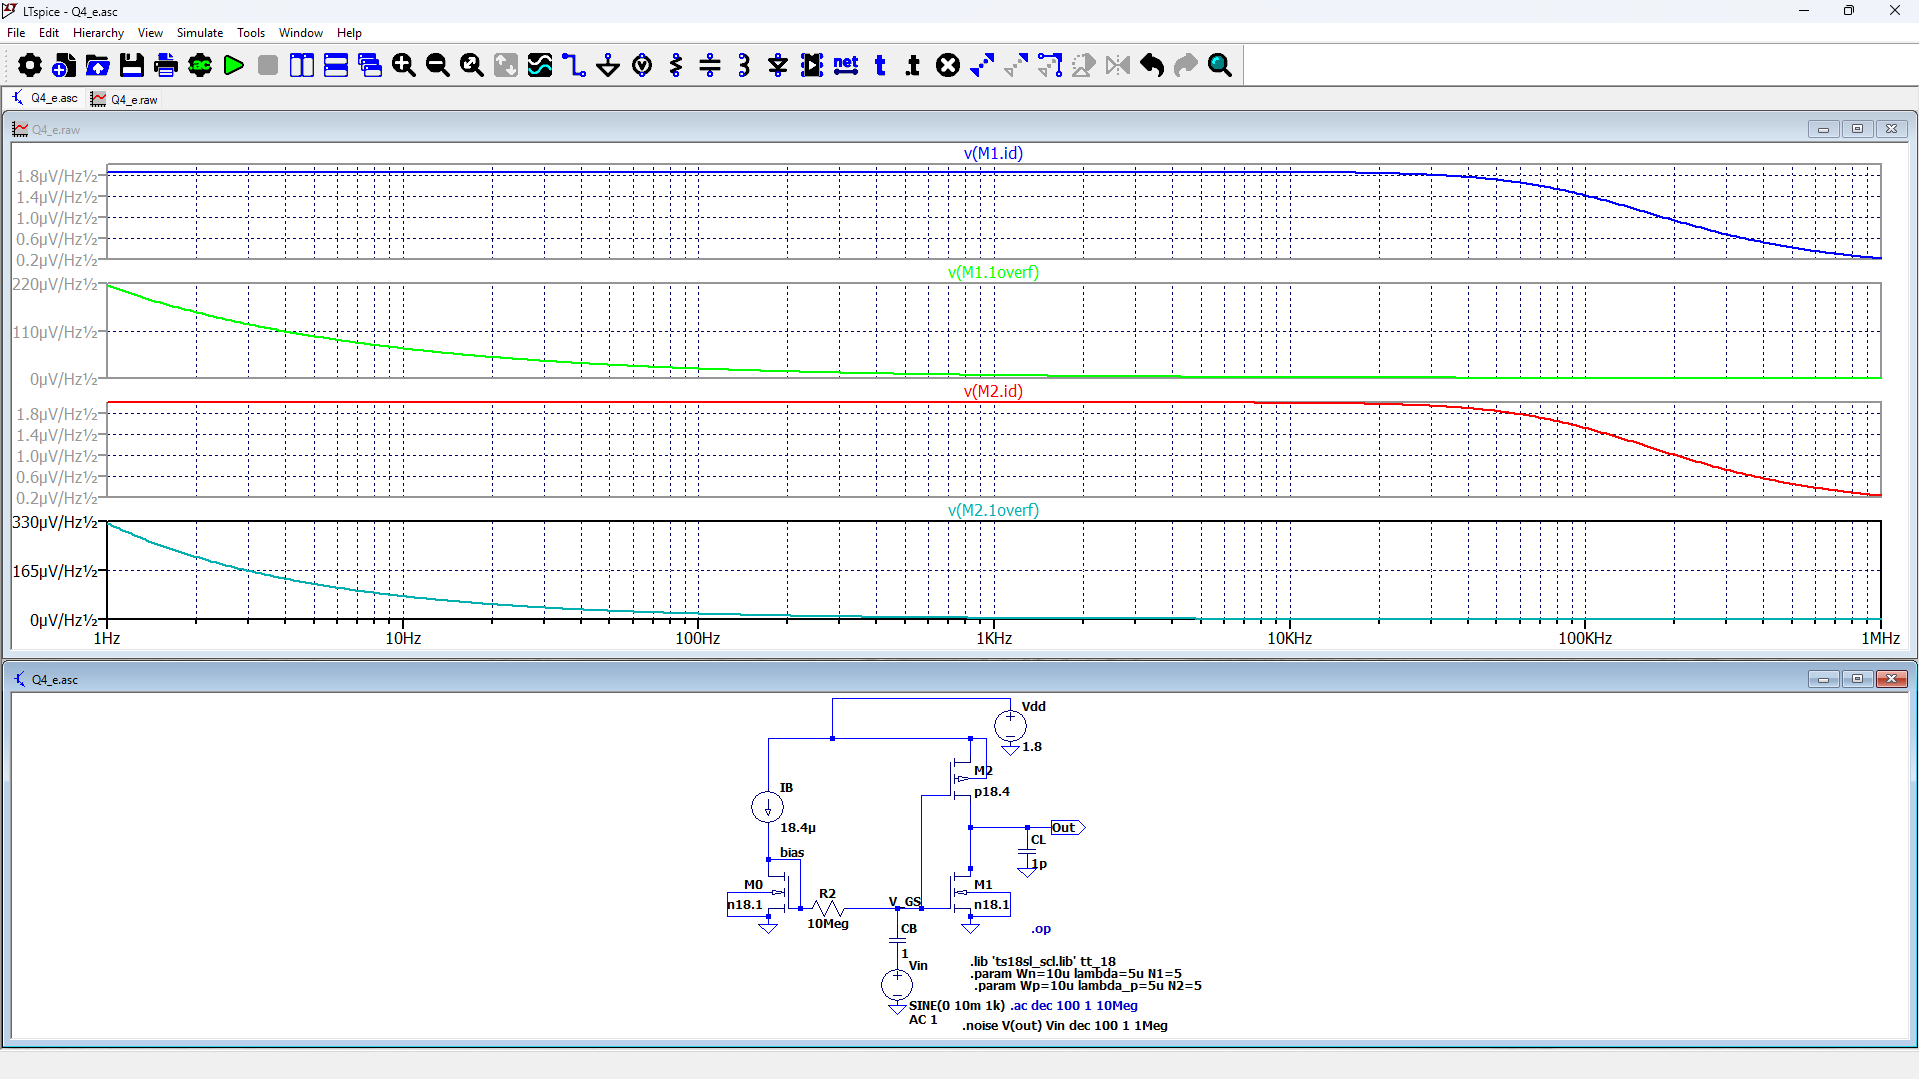
\includegraphics[width=0.8\textwidth]{images/q4_e_3_3.png}
    \caption{Noise PSD of M1 and M2 for the modified design with $W/L = 10\mu/10\mu$.}
\end{figure}

\begin{table}[H]
    \centering
    \caption{Performance Metrics of the Proposed Inverter-Based Amplifier}
    \renewcommand{\arraystretch}{1.4}
    \resizebox{\textwidth}{!}{
    \begin{tabular}{@{}cccccc@{}}
        \toprule
        \textbf{Design} & \textbf{New Gain (V/V)} & \textbf{Amp BW (-3-dB)} & \textbf{$I_{DC}$} & \textbf{New $v_{n_{in,rms}}$} & \textbf{New NEF} \\
        \midrule
        1 ($0.18\mu$) & $25.91$  & $4.198 \text{ MHz}$  & $109.30 \ \mu\text{A}$ & $139.00 \ \mu\text{V}$ & $\mathbf{27.35}$ \\
        2 ($1\mu$)    & $105.03$ & $1.062 \text{ MHz}$  & $112.06 \ \mu\text{A}$ & $17.75 \ \mu\text{V}$  & $\mathbf{7.03}$ \\
        3 ($10\mu$)   & $632.39$ & $114.84 \text{ kHz}$ & $107.91 \ \mu\text{A}$ & $2.37 \ \mu\text{V}$   & $\mathbf{2.80}$ \\
        \bottomrule
    \end{tabular}}
\end{table}

\textbf{Conclusion and Trade-off Analysis:} \\
\begin{table}[H]
    \centering
    \caption{NEF Comparison: Original vs. Modified Topology}
    \renewcommand{\arraystretch}{1.2}
    \begin{tabular}{@{}ccc@{}}
        \toprule
        \textbf{Device Sizing} & \textbf{Original NEF} & \textbf{Modified NEF} \\
        \midrule
        $0.18\mu / 0.18\mu$ & 58.80 & \textbf{27.35} \\
        $1\mu / 1\mu$       & 17.98 & \textbf{7.03} \\
        $10\mu / 10\mu$     & 6.16  & \textbf{2.80} \\
        \bottomrule
    \end{tabular}
\end{table}

The empirical data definitively proves the superiority of the inverter-based topology for noise-efficient design. By carefully sizing the PMOS load to compensate for mobility differences and biasing the inverter exactly at its maximum-gain threshold, the NEF was reduced by more than 50\% across all cases. The current-reused topology successfully multiplied the mid-band voltage gain while drawing identical static current ($I_{DC} \approx 110 \ \mu\text{A}$). While the added gate capacitance of the PMOS device caused a minor reduction in the operational bandwidth, the massive improvements in gain and input-referred noise drastically outweighed the bandwidth penalty, culminating in a highly optimized Noise Efficiency Factor of 2.80 for the $10\mu$ topology.

\end{document}